% Phase 1 Learning Guide — personal study document, NOT a graded deliverable.
% Compile: xelatex Phase1_Learning_Guide.tex (run 2x for ToC)
\documentclass[11pt]{report}

\usepackage[margin=1in]{geometry}
\usepackage{amsmath}
\usepackage{amssymb}
\usepackage{fontspec}
\usepackage{graphicx}
\usepackage{booktabs}
\usepackage{longtable}
\usepackage{array}
\usepackage{xcolor}
\usepackage{caption}
\usepackage{enumitem}
\usepackage{tikz}
\usetikzlibrary{arrows.meta,positioning,shapes.geometric,fit,backgrounds}
\usepackage[most]{tcolorbox}
\usepackage{listings}
\usepackage{titlesec}
\usepackage{fancyhdr}
\PassOptionsToPackage{hyphens}{url}
\usepackage[colorlinks=true,linkcolor=blue!50!black,urlcolor=blue!50!black,citecolor=blue!50!black]{hyperref}
\emergencystretch=3em
\sloppy

\newfontfamily\devanagarifont{Nirmala UI}
\newcommand{\dn}[1]{{\devanagarifont #1}}

% ---------------------------------------------------------------------
% Colors
% ---------------------------------------------------------------------
\definecolor{hindiblue}{HTML}{1F6F8B}
\definecolor{nepalipurple}{HTML}{7A4FA3}
\definecolor{conceptgreen}{HTML}{2E8B57}
\definecolor{warnred}{HTML}{C0392B}
\definecolor{examplegold}{HTML}{B8860B}
\definecolor{codegray}{HTML}{F5F5F5}
\definecolor{titlenavy}{HTML}{102A43}

% ---------------------------------------------------------------------
% Section styling
% ---------------------------------------------------------------------
\titleformat{\chapter}[display]
  {\normalfont\huge\bfseries\color{titlenavy}}
  {\chaptertitlename\ \thechapter}{20pt}{\Huge}
\titleformat{\section}
  {\normalfont\Large\bfseries\color{titlenavy}}{\thesection}{1em}{}
\titleformat{\subsection}
  {\normalfont\large\bfseries\color{hindiblue}}{\thesubsection}{1em}{}

\pagestyle{fancy}
\fancyhf{}
\fancyhead[L]{\small\textit{Phase 1 Learning Guide}}
\fancyhead[R]{\small\leftmark}
\fancyfoot[C]{\thepage}
\renewcommand{\headrulewidth}{0.4pt}

% ---------------------------------------------------------------------
% Callout boxes
% ---------------------------------------------------------------------
\newtcolorbox{concept}[1]{colback=conceptgreen!6,colframe=conceptgreen,
  fonttitle=\bfseries,coltitle=white,colbacktitle=conceptgreen,
  title={\textbf{Concept: #1}},sharp corners=south,boxrule=1pt,left=2mm,right=2mm}

\newtcolorbox{implementation}[1]{colback=hindiblue!6,colframe=hindiblue,
  fonttitle=\bfseries,coltitle=white,colbacktitle=hindiblue,
  title={\textbf{In this project: #1}},sharp corners=south,boxrule=1pt,left=2mm,right=2mm}

\newtcolorbox{example}[1]{colback=examplegold!8,colframe=examplegold,
  fonttitle=\bfseries,coltitle=white,colbacktitle=examplegold,
  title={\textbf{Example: #1}},sharp corners=south,boxrule=1pt,left=2mm,right=2mm}

\newtcolorbox{notebox}[1][Note]{colback=gray!8,colframe=gray!60!black,
  fonttitle=\bfseries,left=2mm,right=2mm,title={\textbf{#1}}}

\newtcolorbox{warnbox}[1][Warning]{colback=warnred!8,colframe=warnred,
  fonttitle=\bfseries,coltitle=white,colbacktitle=warnred,
  left=2mm,right=2mm,title={\textbf{#1}}}

\newtcolorbox{qabox}[1]{colback=nepalipurple!5,colframe=nepalipurple,
  fonttitle=\bfseries,coltitle=white,colbacktitle=nepalipurple,
  title={\textbf{Q: #1}},sharp corners=south,boxrule=1pt,left=2mm,right=2mm,
  breakable}

\lstset{
  backgroundcolor=\color{codegray},
  basicstyle=\ttfamily\small,
  breaklines=true,
  frame=single,
  rulecolor=\color{gray!50},
  showstringspaces=false,
  columns=fullflexible,
}

\newcommand{\fig}[3]{%
  \begin{figure}[htbp]
    \centering
    \includegraphics[width=0.8\textwidth]{../../report/phase1/figures/#1}
    \caption{#2}
    \label{fig:#3}
  \end{figure}
}

\title{\Huge\textbf{Phase 1 — Complete Learning Guide}\\[0.3cm]
\Large Hindi (Model H) and Nepali (Model L)\\[0.2cm]
\large Data Collection, Cleaning, and Tokenizer Construction, Explained From Scratch}
\author{Swaraj Kumar \\ \small 2025202016 \\[0.2cm]
\small \textit{Personal study document --- not a graded deliverable}}
\date{\today}

\begin{document}
\maketitle

\begin{tcolorbox}[colback=gray!8,colframe=gray!50!black,title={\textbf{What this document is}}]
This is a self-study guide, written for myself, so that I can explain
every part of my actual Phase 1 work confidently in a TA evaluation. It is
\textbf{not} a course deliverable and does not affect grading. Every
number in it comes from a real file this project actually produced ---
nothing is invented, and where something was not implemented, this
document says so plainly instead of pretending otherwise. The graded
report is \texttt{report/phase1/phase1\_report.md} / \texttt{.tex} /
\texttt{.pdf}; this document goes deeper, into theory and file-by-file
mechanics, for my own understanding.
\end{tcolorbox}

\tableofcontents

% =======================================================================
\chapter{Introduction: What This Project Is, and Why}
% =======================================================================

\section{The assignment, in plain words}

The course is called \textit{Language Models and Agents}. The individual
project asks every student to build \textbf{two completely independent
Transformer language models from scratch} -- meaning: write the model
architecture yourself in PyTorch (no pretrained models, no HuggingFace
model classes), collect your own training data, train your own tokenizer,
and eventually train and evaluate two separate models.

\begin{concept}{Why two models, not one?}
Because the whole point of the project is to see how a language model's
behaviour changes with the amount of training data available. One model
("Model H") gets a \textbf{higher-resource} language -- one where lots of
clean text already exists on the internet. The other ("Model L") gets a
\textbf{lower-resource} language -- one where good text is scarce and has
to be partly collected by hand. Comparing the two later (Phase 2/3) is
the actual point of the exercise; Phase 1 is just building the raw
material both models will eventually train on.
\end{concept}

\begin{implementation}{Language choice}
\textbf{Model H = Hindi.} Hindi has an enormous amount of public text
available (Wikipedia, curated corpora, web crawls), so \raggedright reaching a large
token count is realistic almost entirely from public sources.

\textbf{Model L = Nepali.} Nepali is on the assignment's fixed allowed
list of lower-resource languages (Assamese, Bhojpuri, Bodo, Dogri,
Konkani, Maithili, Manipuri, Mizo, Nepali, Sindhi). \textbf{Important
personal note:} this project's \textit{original} choice for Model L was
\textbf{Bhojpuri}, and Bhojpuri was fully built, cleaned, and tokenized
before Nepali replaced it once Nepali's own pipeline turned out to have
enough public data to clear every target more comfortably. Bhojpuri's
code has since been removed from the repository, but its numbers are
still in the report as history -- see Chapter~\ref{chap:limitations} for
the full story, so this is not glossed over.
\end{implementation}

\section{What Phase 1 actually delivers}

Phase 1 is \textbf{only} about data and the tokenizer -- not the model
itself. Concretely, for each language, Phase 1 must produce:

\begin{enumerate}
\item Scripts that collect raw text (both from the public internet and by
manual effort).
\item A cleaning pipeline that turns messy raw text into a usable corpus.
\item A statistics report describing what was collected and how it was
cleaned.
\item Train / validation / test splits of that cleaned corpus.
\item A trained subword tokenizer (and the code that trained it).
\end{enumerate}

\begin{notebox}
Nothing about the neural network itself exists yet. There is no
\texttt{model.py}, no training loop, no PyTorch \texttt{nn.Module}. That
is Phase 2. If a TA asks "so where's the Transformer?" the honest answer
for Phase 1 is: it doesn't exist yet, by design -- this phase is the data
foundation the model will be trained on later.
\end{notebox}

\section{The two pipelines, and why they look completely different}

This is one of the most important things to understand about this
project, and also the thing most likely to confuse a first read of the
code: \textbf{Hindi and Nepali are built by two genuinely different
pieces of software}, not one script parameterised by language.

\begin{center}
\begin{tabular}{p{4cm}p{5.5cm}p{5.5cm}}
\toprule
& \textbf{Hindi} & \textbf{Nepali} \\
\midrule
Style & Single-pass cleaner: one script reads raw text and writes cleaned
text in one straight run & Stage-based pipeline: 15 numbered stages
(S00--S14), each its own script, each with its own checkpoint \\
Code location & \texttt{hindi/data/pipeline/} + \texttt{scripts/clean\_lib.py} &
\texttt{nepali/scripts/} + its own \texttt{corpuslib} package \\
Dedup method & Exact hash only & Exact hash \textit{and} MinHash/LSH
near-duplicate detection \\
Language filter & \texttt{langdetect} + a hand-written Bhojpuri-marker
check & \texttt{fastText} with a margin-based decision \\
Tokenizer & SentencePiece Unigram & SentencePiece BPE \\
\bottomrule
\end{tabular}
\end{center}

\begin{warnbox}[A detail that looks like a bug but isn't]
Every Nepali stage script's docstring shows its example command as
\texttt{python hindi/scripts/sXX.py} -- but there is no
\texttt{hindi/scripts/} directory anywhere in this repository. This is
leftover template text: the \texttt{corpuslib} framework was designed so
that \textit{both} languages could share it, with Hindi meant to be the
"source of truth" copy and Nepali a synced copy (see
\texttt{run\_pipeline.py}'s \texttt{sync} subcommand, which explicitly
refuses to run from Nepali's side because "nepali is a copy, not the
source"). In practice, that dual-language plan was never finished --
Hindi kept its earlier, separate pipeline instead, and only Nepali
actually uses this stage-based framework. If you go looking for
\texttt{hindi/scripts/} because a docstring mentioned it, you won't find
it, and that's expected.
\end{warnbox}

% =======================================================================
\chapter{Core Theory: The Ideas Behind Every Stage}
% =======================================================================

This chapter explains every concept used in this project \textbf{from
zero} -- assume you have never heard the term before. Each concept is
followed by exactly how it shows up in this project's actual code.

\section{What is a corpus?}

\begin{concept}{Corpus}
A \textbf{corpus} (plural: corpora) is just a large collection of text
used to train or study a language model. It's not one document -- it's
potentially millions of documents (news articles, Wikipedia pages,
books, social media posts) put together. The quality and size of the
corpus is the single biggest factor in how good a trained language
model ends up being -- more so than almost any architecture choice made
later in Phase 2.
\end{concept}

\begin{implementation}{This project's two corpora}
Hindi's corpus, after cleaning, is 704,101 documents / 1,764,596,782
characters. Nepali's, after its full pipeline, is 1,918,265 documents /
635,204,333 tokens. Both are stored as one text file per document plus a
metadata file (Hindi) or as line-delimited JSON files, one JSON object
per document (Nepali) -- two different storage conventions, again
because the two pipelines were built independently.
\end{implementation}

\section{Manual vs. downloaded collection, and the 20\% rule}

\begin{concept}{Why "manual" data matters}
Anyone can write a script that downloads an existing dataset from Hugging
Face. That is fast, but it does not demonstrate that a student can
actually go out and \textit{build} a dataset -- find sources, extract
text, clean up formatting, deal with things not already packaged for
machine learning. The assignment requires that \textbf{at least 20\% of
the final training tokens, for both languages, come from manual
collection} -- meaning collection work beyond "point a downloader at an
existing dataset."
\end{concept}

\begin{example}{What counts as manual, what doesn't}
Downloading \texttt{wikimedia/wikipedia} from Hugging Face: \textbf{not}
manual -- it's already a packaged dataset someone else prepared.
Downloading the raw Wikipedia XML dump yourself from
\texttt{dumps.wikimedia.org} and running it through WikiExtractor
yourself: \textbf{is} manual, even though the underlying text is the same
Wikipedia content -- because you did the extraction work, not Hugging
Face. This exact distinction is why \texttt{hindi/data/pipeline/
ingest\_wikipedia\_dump.py} exists as a separate script from
\texttt{download\_hindi.py}: same content, different collection method,
different \texttt{source\_type} label.
\end{example}

\begin{implementation}{Where manual/downloaded is tracked}
Every single document, from the moment it's collected, carries a
\texttt{source\_type} field (\texttt{"manual"} or \texttt{"downloaded"})
in its metadata. This field survives all the way through cleaning to the
final corpus, so the manual percentage can always be recomputed directly
from real data rather than trusted as a remembered number.
\texttt{scripts/validate\_phase1.py} (Hindi) and
\texttt{scripts/validate\_phase1\_nepali.py} (Nepali) both compute this
percentage fresh, from the actual files, every time they run.

Hindi ended at 28.65\% manual (by characters). Nepali ended at 26.41\%
manual (by tokens -- Nepali's pipeline tracks tokens/words per lane, not
characters, so its manual percentage is measured in a different unit;
this is disclosed honestly in the report rather than papered over).
\end{implementation}

\section{Unicode normalization: NFC vs.\ NFKC}

\begin{concept}{Why text needs "normalizing" at all}
The same visual character can sometimes be represented by more than one
sequence of underlying bytes in Unicode. For example, a character with an
accent mark can be stored as one single "precomposed" code point, or as
two separate code points (the base letter, then a combining accent mark)
that render identically on screen. If two documents contain the "same"
text but encoded differently, a computer comparing them byte-for-byte
would wrongly think they're different -- and any deduplication step would
fail to catch the duplicate. \textbf{Normalization} picks one canonical
encoding so equivalent text always looks byte-identical.
\end{concept}

\begin{concept}{NFC vs.\ NFKC -- the difference that matters here}
\textbf{NFC} (Normalization Form Canonical Composition) merges
code-point sequences into their single composed form where possible, but
preserves every character's actual identity and meaning.
\textbf{NFKC} (Normalization Form Compatibility Composition) goes
further -- it also converts characters that are visually/semantically
"compatible" into a simpler form (e.g.\ turning a stylized character
variant into a plain one), which can \textit{change} the text, not just
re-encode it identically.
\end{concept}

\begin{example}{Why NFKC is dangerous for Devanagari}
Devanagari script (used by both Hindi and Nepali) uses two special
invisible characters: \textbf{ZWNJ} (zero-width non-joiner, U+200C) and
\textbf{ZWJ} (zero-width joiner, U+200D). These control whether two
consecutive consonants visually merge into a single combined "conjunct"
glyph or stay drawn as two separate letters -- this is a real,
meaningful spelling distinction in Devanagari, not decoration. NFKC's
"compatibility" normalization can strip or alter these, silently changing
how a word is actually spelled. NFC does not touch them.
\end{example}

\begin{implementation}{This project's choice}
Both pipelines use \textbf{NFC, never NFKC}. Hindi's
\texttt{clean\_lib.py:normalize\_text()} calls
\texttt{unicodedata.normalize("NFC", text)} and then strips only
zero-width/control characters that are \textit{not} ZWJ/ZWNJ (the regex
\texttt{\_ZERO\_WIDTH\_AND\_CONTROL} explicitly excludes them). Nepali's
\texttt{corpuslib/textnorm.py} makes the same choice, and even lets
\texttt{configs/language.yaml} decide per-language whether to strip
joiners at all (Hindi's config strips some; Nepali's does not, since ZWJ
is load-bearing inside real Nepali conjuncts like
\dn{पुर्‍याउने}).
\end{implementation}

\section{Language identification (Language ID / LID)}
\label{sec:concept-langid}

\begin{concept}{What language ID does}
Language identification is the task of automatically detecting which
human language a piece of text is written in. This sounds simple but is
genuinely hard when two languages share the same script and a lot of
vocabulary -- exactly the situation between Hindi and Nepali (and
historically, Hindi and Bhojpuri), since all three are written in
Devanagari and share many common words.
\end{concept}

\begin{concept}{Confidence vs.\ margin}
A language-ID model doesn't just say "this is Hindi" -- it gives a
probability for every language it knows. A naive approach accepts a
document if its top-predicted language's probability is above some
threshold (e.g.\ 85\%). The problem: for two very similar languages, a
model can be, say, 60\% confident it's Hindi and 55\% confident it's
Nepali -- neither passes a raw-confidence threshold cleanly, but the
\textbf{margin} between them (the gap between the top language's
probability and the next-best competing language's probability) is a
much more informative signal of genuine ambiguity than either raw number
alone.
\end{concept}

\begin{implementation}{Two different approaches, by necessity}
Hindi's pipeline uses Python's \texttt{langdetect} library, which
\textbf{has no label for Bhojpuri at all} -- it cannot classify text as
Bhojpuri even if that's genuinely what it is, so it will happily call
real Bhojpuri text "Hindi." To close that gap, Hindi's
\texttt{clean\_lib.py} adds a second, hand-written check: a list of
common Bhojpuri words (\dn{बा}, \dn{बाटे}, \dn{गइल}, etc.) versus common
Hindi words (\dn{है}, \dn{हैं}, \dn{गया}, etc.) -- if Bhojpuri markers
clearly outnumber Hindi markers, the document is rejected before
\texttt{langdetect} even gets a say.

Nepali's pipeline uses \texttt{fastText}'s \texttt{lid.176} model
instead, and explicitly computes the \textbf{margin} between Nepali's
score and the best competing Devanagari-script language (Hindi, Maithili,
Sanskrit, etc.) -- see \texttt{corpuslib/langid.py}. This is a more
principled version of the same underlying problem Hindi's marker-list
check is trying to solve by hand.

\begin{warnbox}
An earlier version of this exact pipeline had a language-ID bug that
deleted \textbf{94\% of a corpus silently}: the \texttt{fastText} library
crashed on a NumPy version incompatibility, the crash was caught by a
blanket \texttt{except Exception}, and every document was treated as
"rejected" -- while the run still logged \texttt{SUCCESS}. This is
exactly why \texttt{nepali/scripts/s00\_doctor.py} exists: it tests every
dependency actually works \textit{before} a multi-hour run starts, and
\texttt{s04\_langid.py} now \textbf{aborts loudly} (rather than silently
continuing) if the fraction of documents kept falls outside an expected
band configured in \texttt{language.yaml}.
\end{warnbox}
\end{implementation}

\section{Deduplication: exact vs.\ near-duplicate}

\begin{concept}{Why duplicate documents are a problem}
If the same document (or a slightly reformatted copy of it) appears
multiple times in a training corpus, the model effectively sees that text
more often than it should, which can make it memorize that specific text
rather than learning general language patterns. Large web-crawled
datasets are full of duplicates -- the same news article gets
re-published on multiple sites, the same product description appears on
a hundred pages, etc.
\end{concept}

\begin{concept}{Exact-hash deduplication}
The simplest approach: normalize each document's text (lowercase,
collapse whitespace, strip punctuation), then compute a hash (a short
fixed-length fingerprint) of the result. Two documents with the same hash
are (almost certainly) exact duplicates once formatting differences are
ignored. This is fast and simple, but misses documents that are
\textit{almost} the same but not byte-identical after normalization --
e.g.\ the same article with one paragraph added.
\end{concept}

\begin{concept}{Near-duplicate detection: MinHash + LSH}
To catch documents that are similar but not identical, this project uses
\textbf{MinHash} combined with \textbf{LSH (Locality-Sensitive
Hashing)}.

\textit{MinHash}, step by step: break a document into overlapping chunks
of $n$ consecutive words (called \textbf{shingles}, e.g.\ 5-word
windows). Apply many different hash functions (this project uses 100) to
the whole set of shingles, and for each hash function keep only the
\textit{minimum} hash value it produced. The resulting 100 numbers are
that document's "signature." The mathematical guarantee is: the fraction
of matching numbers between two documents' signatures is a good estimate
of their real word-overlap similarity (the \textbf{Jaccard similarity}
of their shingle sets) -- without ever needing to compare the full texts
against each other directly.

\textit{LSH} then makes this scale to millions of documents: instead of
comparing every document's signature against every other document's
signature (which would be far too slow), the 100-number signature is
split into bands (this project: 20 bands of 5 numbers each), and two
documents are only ever compared for real if they land in the exact same
bucket for at least one band. Similar documents are very likely to share
at least one band; wildly different documents almost never do.
\end{concept}

\begin{example}{Working through it with small numbers}
Say a document has the shingles (3-word windows) \{"ram went home",
"went home today"\}. Apply hash function \#1 to both shingles, keep
whichever result is smaller -- that's the document's MinHash value \#1.
Repeat with 99 more hash functions. Two documents whose text overlaps
heavily will keep landing on the same minimum value for many of those
100 hash functions purely because they share most of the same shingles
to begin with -- that's the whole trick.
\end{example}

\begin{implementation}{Where this runs, and the manual-priority rule}
Nepali's \texttt{corpuslib/dedup.py} implements exactly this: 100
permutations, 20 bands of 5 rows, a similarity threshold of 0.55,
5-word shingles. It runs twice: once in \texttt{s08\_dedup.py} (removing
duplicates \textit{within} the corpus itself) and once in
\texttt{s09\_decontaminate.py} (checking that no training document is a
near-duplicate of something already held out for validation/test --
otherwise the model could effectively "see" its own test answers during
training).

Hindi's pipeline only does \textbf{exact-hash} deduplication
(\texttt{clean\_lib.py:dedup\_key()}) -- it does not run MinHash/LSH at
all. This is a real, acknowledged asymmetry between the two pipelines
(Section~\ref{sec:limitations-summary}), not a hidden gap.

\textbf{One deliberate rule in both languages' dedup logic}: when a
duplicate is found between a manually-collected copy and a
downloaded copy of the same text, \textbf{the manual copy always wins}
and the downloaded copy is the one removed. Manual data is the scarce
resource this project has to protect (it's what the 20\% floor is
measuring) -- a "blind" dedup pass that didn't care which copy came from
which lane could silently erode the manual percentage by deleting manual
copies at random.
\end{implementation}

\section{Tokenization: turning text into model input}

\begin{concept}{Why models can't just read raw text}
A neural network needs its input broken into a finite, fixed set of
discrete units called \textbf{tokens}, each mapped to a number (an
"embedding" index). You could use whole words as tokens, but that means
the vocabulary has to include every possible word form ever
seen -- infeasible for morphologically rich languages like Hindi/Nepali,
where a single root word can take dozens of suffixed forms. The modern
answer is \textbf{subword tokenization}: break words into smaller,
reusable pieces, so a large vocabulary of \textit{whole} words is
replaced by a much smaller vocabulary of \textit{parts} that can be
recombined.
\end{concept}

\begin{concept}{Byte Pair Encoding (BPE)}
BPE builds its vocabulary greedily: start with every individual character
as a token. Repeatedly find the \textbf{most frequent adjacent pair} of
existing tokens in the training corpus and merge that pair into one new
token. Stop once the vocabulary reaches the target size. The key
limitation: once two tokens are merged, that decision is
\textbf{permanent} -- BPE never revisits an earlier merge even if a
later merge would have been a better overall segmentation.
\end{concept}

\begin{example}{BPE merges, step by step}
Suppose the corpus has many occurrences of the word \dn{"लड़का"} (boy). BPE
might first merge the two most frequent adjacent characters into one
token, then merge that new token with the next most frequent neighbor,
and so on -- e.g.\ \dn{ल}+\dn{ड़} $\rightarrow$ \dn{लड़}, then
\dn{लड़}+\dn{का} $\rightarrow$ \dn{लड़का} becomes one single token once
merges reach that far, \textit{if} \dn{"लड़का"} was frequent enough in the
training data to earn that many merge steps before the vocabulary budget
runs out.
\end{example}

\begin{concept}{Unigram Language Model tokenization}
Unigram tokenization works differently: instead of building up from
characters via merges, it starts from a large candidate set of possible
subword pieces, then uses the EM (Expectation-Maximization) algorithm to
iteratively estimate a probability for each candidate piece and discard
the least useful ones, repeating until the vocabulary reaches the target
size. Critically, for any given piece of text, Unigram considers the
\textit{whole space} of possible ways to split it into pieces and keeps
whichever segmentation is most probable under the current model -- it
can effectively "reconsider" a segmentation choice that BPE's
one-merge-at-a-time process never revisits.
\end{concept}

\begin{implementation}{Which algorithm each language uses, and why}
\textbf{Hindi uses SentencePiece Unigram.} The argument (documented in
\texttt{report/phase1/phase1\_report.md} \S5): Hindi is a
morphologically rich, agglutinative-suffixing language on top of
Devanagari's conjunct-cluster orthography (where one visual glyph can
correspond to several underlying code points). BPE's inability to revisit
a bad early merge is a real structural weakness for this kind of script;
Unigram's probabilistic re-estimation is a better theoretical fit. This
argument was \textbf{not empirically tested head-to-head on Hindi
specifically} -- it's a structural argument, not a measured one, and the
report says so honestly.

\textbf{Nepali uses SentencePiece BPE}, chosen simply because that's what
\texttt{nepali/configs/tokenizer.yaml} was configured to use as this
pipeline's default -- \textit{not} a considered per-language linguistic
decision. But there's a real safety net: the config includes
\texttt{compare\_unigram.enabled: true}, meaning \textit{if} BPE's
measured fertility (see below) had exceeded 2.10 tokens/word, the
pipeline would automatically also train a Unigram model and keep
whichever scored better. It never triggered -- Nepali's BPE fertility
stayed at 1.48--1.70 across the whole sweep, comfortably under that
threshold -- so this is a genuine comparison that was set up and simply
didn't end up mattering, not an untested assumption.
\end{implementation}

\begin{concept}{Fertility, chars/token, and vocabulary utilization}
\textbf{Fertility} = average number of tokens produced per whitespace-
delimited word. Lower fertility means the tokenizer represents text more
compactly (fewer tokens for the same content) -- generally desirable,
since it means more effective context length and less computation per
unit of real text, but a fertility that's too low can mean the tokens
are too coarse-grained to generalize well.

\textbf{Characters per token} is a related, more granular measure of
compactness.

\textbf{Vocabulary utilization} = the fraction of the tokenizer's
vocabulary that actually gets used at least once on held-out text. A
vocabulary size larger than the language's real subword diversity wastes
embedding-table parameters on pieces that are rarely or never emitted.
\end{concept}

\begin{implementation}{The actual trade-off that decided vocab size}
Both languages were capped to a vocabulary size between 5,000 and 10,000
by a course-TA ruling, because a much larger vocabulary (e.g.\ 24,000)
would make the embedding table alone consume roughly half of the whole
$\sim$25M-parameter model budget planned for Phase 2 -- leaving too
little capacity for the actual Transformer layers. Within that
5k--10k range:

\begin{itemize}
\item \textbf{Hindi chose 8,000} on a fertility/embedding-cost trade-off:
fertility kept improving from 5k to 10k, but the gain from 8k$\to$10k
(2.7\% relative) was much smaller than 5k$\to$8k (6.7\% relative), for
meaningfully more embedding cost. Measured directly: 8,000 produced
\textit{more} total tokens than 10,000 (505.9M vs.\ 491.9M), pushing
Hindi to 101.2\% of the 500M planning target instead of 98.4\%.
\item \textbf{Nepali chose 10,000} by its pipeline's own automated rule:
"walk the swept sizes, stop at the first one where growing further buys
less than a 3\% relative fertility gain." No elbow was found within the
swept range at all (fertility kept improving meaningfully all the way to
10,000), so the rule kept the largest candidate.
\end{itemize}
\end{implementation}

\section{Train / validation / test splits, and data leakage}

\begin{concept}{Why three separate splits}
\textbf{Train} is what the model actually learns from. \textbf{Validation}
is used during development to make decisions (like which tokenizer
vocabulary size to pick) without ever touching the final judge of
quality. \textbf{Test} is held back and used only once, at the very end,
to report how well the finished model actually generalizes to text it
has never influenced in any way -- not during training, not during any
tuning decision.
\end{concept}

\begin{concept}{Data leakage}
\textbf{Leakage} happens when information from validation or test data
sneaks into training, or into a decision that shapes training --
directly (the exact same document ends up in two splits) or indirectly
(a near-duplicate of a test document ends up in train, so the model has
effectively already "seen" it in a slightly different wrapper). Leakage
makes evaluation numbers look better than the model's real, honest
capability, which defeats the entire purpose of holding out test data
in the first place.
\end{concept}

\begin{example}{Splitting by document, not by sentence or line}
If you split individual \textit{sentences} from the same article across
train and test, a model can learn stylistic and factual details from one
sentence in train and then look unfairly capable when asked about a
neighboring sentence from the same article in test -- because it isn't
really being tested on unseen content, just an unseen slice of a document
it partly already saw. Both pipelines in this project split at the
\textbf{whole-document} level specifically to avoid this.
\end{example}

\begin{implementation}{How each pipeline actually splits}
\textbf{Hindi} (\texttt{split\_hindi.py}): shuffles all cleaned documents
with a fixed random seed (42), then assigns roughly 96\% to train, 2\% to
validation, 2\% to test, purely by document count. Simple, but it runs
\textit{after} cleaning is fully done, so quality filtering has already
happened to all three splits identically.

\textbf{Nepali} (\texttt{s07\_holdout.py}) does something more careful,
and it's one of the more interesting design choices in this project:
val/test are carved out \textbf{immediately after language-ID
(S04)}, \textit{before} the heuristic quality filter (S05), the
perplexity filter (S06), deduplication (S08), or lane balancing (S10)
ever run. The reasoning: if the same quality filters that \textit{select}
training data also get to \textit{curate} the evaluation set, then
evaluation partly measures "does this model do well on text our own
filters like," not genuine model quality on a fair, representative
sample. \texttt{s05\_heuristics.py} and \texttt{s06\_perplexity.py}
explicitly read S07's leftover \texttt{train\_pool} output, never S04's
output directly -- so val/test genuinely never pass through those
filters. The split itself is a deterministic hash of each document's ID
against a fixed seed (not a shuffle held in memory), so the exact same
split is reproducible from the seed alone, and it scales to a corpus that
doesn't need to fit in memory to be split.
\end{implementation}

\section{Perplexity filtering: measuring how "fluent" text reads}

\begin{concept}{What perplexity means, informally}
Perplexity (or the closely related \textbf{cross-entropy}, its
logarithm) is a measure of how "surprised" a language model is by a
piece of text -- lower means the text follows patterns the model
considers normal and predictable; higher means it's unusual, garbled, or
statistically unlike the kind of text the model was trained to expect. A
small n-gram model trained on clearly \textit{well-written} reference
text can be used as a crude but genuinely useful fluency detector: text
that scores badly against it is more likely to be boilerplate, garbled
extraction artifacts, or other low-quality noise, though it isn't a
perfect signal.
\end{concept}

\begin{implementation}{Nepali's S06 stage}
\texttt{s06\_perplexity.py} trains a simple order-5 word n-gram model
(with "stupid backoff" smoothing) on a sample of documents from sources
already known to be edited prose -- Wikisource, OCR'd books. Every
\textit{other} document (not from those reference sources, to avoid
scoring reference text against itself) gets a perplexity score, and the
worst-scoring 3\% is dropped as the least fluent tail. There's a
built-in sanity check: if the dropped documents' \textit{average length}
turns out to be suspiciously short, that's the signature of a broken
n-gram model flagging near-empty fragments rather than genuinely
disfluent prose -- in that case the whole filter skips itself rather
than dropping real data for a reason that doesn't actually hold up.
\textbf{Hindi's pipeline has no equivalent stage at all} -- this is a
capability only Nepali's pipeline has.
\end{implementation}

\section{Data quality control as a design philosophy}

\begin{concept}{"Fail loudly" vs.\ "fail silently"}
A pipeline that silently drops data on an error (or, worse, silently
accepts \textit{everything} because a filter quietly stopped working) is
far more dangerous than one that stops and complains -- a silent failure
can run for hours and produce a corpus that looks fine on the surface but
is actually badly broken, and nobody notices until much later, if ever.
\end{concept}

\begin{implementation}{This is not theoretical for this project}
The NumPy/fastText incident described in Section~\ref{sec:concept-langid}
(the 94\%-of-corpus-silently-deleted bug) is exactly this failure mode,
and it directly shaped how the Nepali pipeline is built now:
\texttt{s00\_doctor.py} tests every dependency before any expensive run
starts; \texttt{s03\_normalize.py} is designed so it can \textit{never}
drop a document (only later stages are allowed to decide "good" vs.
"bad", so retention numbers can always be attributed to one specific,
identifiable cause); and \texttt{s04\_langid.py}/\texttt{s05\_heuristics.py}
both check their own retention rate against an expected band from config
and \textbf{abort the whole run} if it falls outside that band, rather
than silently continuing on data that's probably wrong.
\end{implementation}

% =======================================================================
\chapter{The Complete Pipeline, End to End}
% =======================================================================

\section{Big-picture flowchart}

\begin{center}
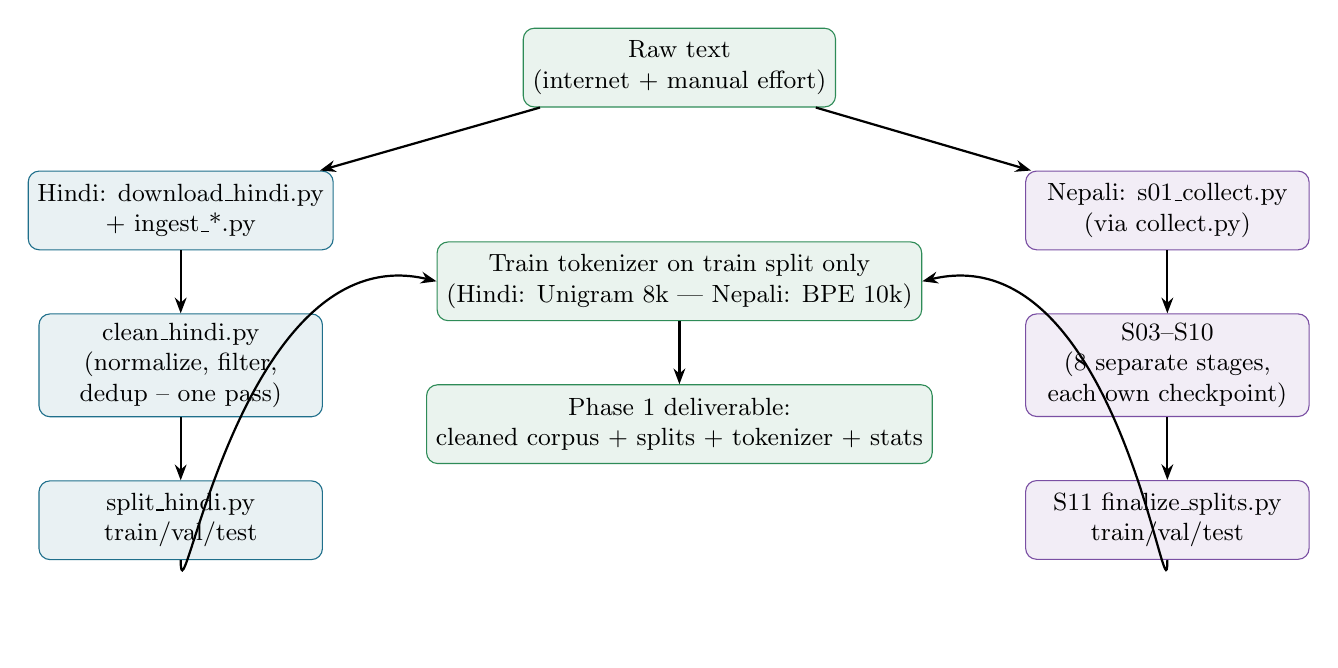
\begin{tikzpicture}[
  node distance=8mm and 12mm,
  box/.style={rectangle, rounded corners, draw=black!60, fill=gray!8,
    minimum width=3.6cm, minimum height=1cm, align=center, font=\small},
  hbox/.style={box, draw=hindiblue, fill=hindiblue!10},
  nbox/.style={box, draw=nepalipurple, fill=nepalipurple!10},
  cbox/.style={box, draw=conceptgreen, fill=conceptgreen!10},
  arr/.style={-{Stealth[length=2mm]}, thick}
]
\node[cbox] (raw) {Raw text\\(internet + manual effort)};
\node[hbox, below left=of raw, xshift=-1.2cm] (hcollect) {Hindi: download\_hindi.py\\+ ingest\_*.py};
\node[nbox, below right=of raw, xshift=1.2cm] (ncollect) {Nepali: s01\_collect.py\\(via collect.py)};
\node[hbox, below=of hcollect] (hclean) {clean\_hindi.py\\(normalize, filter,\\dedup -- one pass)};
\node[nbox, below=of ncollect] (nstage) {S03--S10\\(8 separate stages,\\each own checkpoint)};
\node[hbox, below=of hclean] (hsplit) {split\_hindi.py\\train/val/test};
\node[nbox, below=of nstage] (nsplit) {S11 finalize\_splits.py\\train/val/test};
\node[cbox, below=17mm of raw] (tok) {Train tokenizer on train split only\\(Hindi: Unigram 8k | Nepali: BPE 10k)};
\node[cbox, below=of tok] (final) {Phase 1 deliverable:\\cleaned corpus + splits + tokenizer + stats};

\draw[arr] (raw) -- (hcollect);
\draw[arr] (raw) -- (ncollect);
\draw[arr] (hcollect) -- (hclean);
\draw[arr] (ncollect) -- (nstage);
\draw[arr] (hclean) -- (hsplit);
\draw[arr] (nstage) -- (nsplit);
\draw[arr] (hsplit.south) .. controls +(0,-1) and +(-2.5,0.6) .. (tok.west);
\draw[arr] (nsplit.south) .. controls +(0,-1) and +(2.5,0.6) .. (tok.east);
\draw[arr] (tok) -- (final);
\end{tikzpicture}
\end{center}

\section{Nepali's stage order, drawn out}

The file numbers (S00\ldots S14) do \textbf{not} match execution order --
S07 genuinely runs before S05/S06, on purpose (Section~5.8). This diagram
shows the \textit{real} order.

\begin{center}
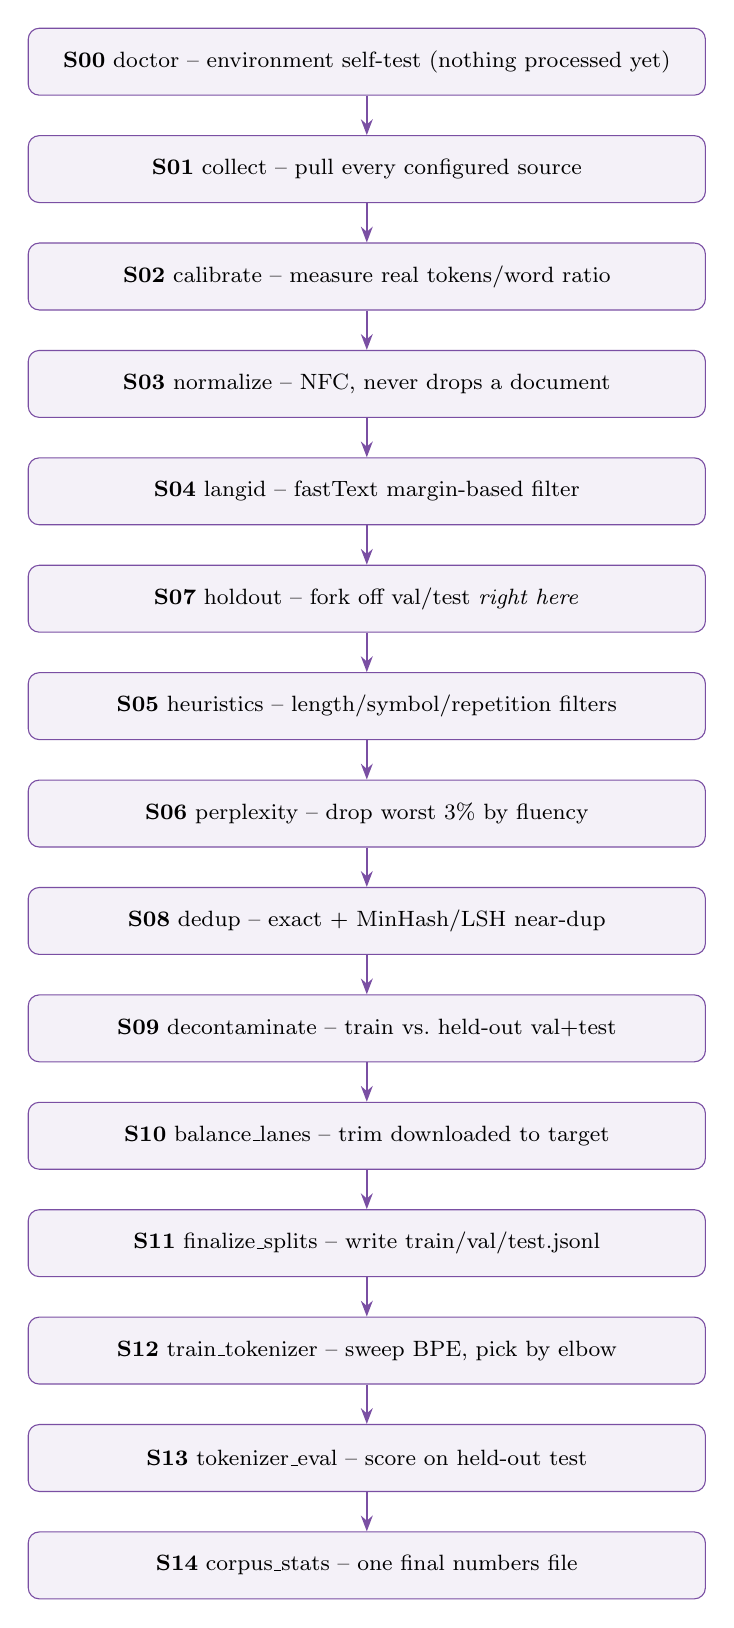
\begin{tikzpicture}[
  node distance=5mm,
  sbox/.style={rectangle, rounded corners, draw=nepalipurple, fill=nepalipurple!8,
    minimum width=8.6cm, minimum height=0.85cm, align=left, font=\footnotesize},
  arr/.style={-{Stealth[length=2mm]}, thick, nepalipurple}
]
\node[sbox] (s00) {\textbf{S00} doctor -- environment self-test (nothing processed yet)};
\node[sbox, below=of s00] (s01) {\textbf{S01} collect -- pull every configured source};
\node[sbox, below=of s01] (s02) {\textbf{S02} calibrate -- measure real tokens/word ratio};
\node[sbox, below=of s02] (s03) {\textbf{S03} normalize -- NFC, never drops a document};
\node[sbox, below=of s03] (s04) {\textbf{S04} langid -- fastText margin-based filter};
\node[sbox, below=of s04] (s07) {\textbf{S07} holdout -- fork off val/test \textit{right here}};
\node[sbox, below=of s07] (s05) {\textbf{S05} heuristics -- length/symbol/repetition filters};
\node[sbox, below=of s05] (s06) {\textbf{S06} perplexity -- drop worst 3\% by fluency};
\node[sbox, below=of s06] (s08) {\textbf{S08} dedup -- exact + MinHash/LSH near-dup};
\node[sbox, below=of s08] (s09) {\textbf{S09} decontaminate -- train vs.\ held-out val+test};
\node[sbox, below=of s09] (s10) {\textbf{S10} balance\_lanes -- trim downloaded to target};
\node[sbox, below=of s10] (s11) {\textbf{S11} finalize\_splits -- write train/val/test.jsonl};
\node[sbox, below=of s11] (s12) {\textbf{S12} train\_tokenizer -- sweep BPE, pick by elbow};
\node[sbox, below=of s12] (s13) {\textbf{S13} tokenizer\_eval -- score on held-out test};
\node[sbox, below=of s13] (s14) {\textbf{S14} corpus\_stats -- one final numbers file};
\foreach \a/\b in {s00/s01, s01/s02, s02/s03, s03/s04, s04/s07, s07/s05,
                   s05/s06, s06/s08, s08/s09, s09/s10, s10/s11, s11/s12,
                   s12/s13, s13/s14}
  \draw[arr] (\a) -- (\b);
\end{tikzpicture}
\end{center}

% =======================================================================
\chapter{Hindi Pipeline, File by File}
% =======================================================================

\section{Overview}

Hindi's pipeline is five scripts plus one shared library, run one after
another by hand (no orchestrator script ties them together the way
Nepali's \texttt{run\_pipeline.py} does):

\begin{center}
\begin{tabular}{lll}
\toprule
Order & File & Purpose \\
\midrule
1 & \texttt{download\_hindi.py} & Pull public sources (Wikipedia, Sangraha, FineWeb-2) \\
2 & \texttt{ingest\_manual.py} & Register typed/OCR'd/PDF/scraped manual text \\
2 & \texttt{ingest\_wikipedia\_dump.py} & Register the self-extracted Wikipedia dump (manual) \\
3 & \texttt{clean\_hindi.py} & Normalize, filter, dedup -- raw $\to$ cleaned \\
4 & \texttt{split\_hindi.py} & Cleaned $\to$ train/validation/test \\
5 & \texttt{train\_tokenizer.py} & Train SentencePiece Unigram \\
6 & \texttt{analyze\_tokenizer.py} & Measure fertility/UNK/coverage on validation \\
\bottomrule
\end{tabular}
\end{center}

\section{download\_hindi.py}

\textbf{Input:} nothing (streams directly from Hugging Face Hub).
\textbf{Output:} \texttt{data/raw/downloaded/\{text/*.txt, metadata.jsonl\}}.

Streams four Hugging Face datasets rather than downloading them in full
(each is far larger than needed): Wikipedia
(\texttt{wikimedia/wikipedia:20231101.hi}), Sangraha's human-verified
Hindi partition, Sangraha's larger but unverified partition, and
FineWeb-2's CommonCrawl-derived Hindi partition. Each source function
stops once it reaches a configurable character budget (defaults: no cap
for Wikipedia since the dump is finite anyway; 300M chars for Sangraha
verified; 500M each for Sangraha unverified and FineWeb-2). FineWeb-2
rows are additionally pre-filtered on the dataset's own
\texttt{language\_score} field ($\geq 0.9$) as a cheap first pass against
CommonCrawl's known Hindi/Bhojpuri labeling noise -- explicitly documented
as \textit{not} a substitute for the real language-ID filter that runs
later in \texttt{clean\_hindi.py}.

Every document gets a stable ID: \texttt{sha1("\{source\_name\}:
\{raw\_id\}")}, truncated to 10 hex characters, prefixed
\texttt{hi\_downloaded\_}. Stable IDs mean re-running with
\texttt{--append} to add a new source never creates accidental
duplicates of sources already on disk.

\section{ingest\_manual.py}

\textbf{Input:} a folder of your own \texttt{.txt} files, or PDFs/images,
or a file listing URLs. \textbf{Output:} same schema as above, written
into \texttt{data/raw/manual/}.

One script, four subcommands, matching the four manual-collection methods
this project's brief allows:

\begin{itemize}[leftmargin=1.4cm]
\item[\texttt{typed}] Registers plain text files you already typed or
transcribed yourself.
\item[\texttt{ocr}] Runs Tesseract OCR over PDFs/images (needs the
Tesseract binary installed separately, plus its Hindi \texttt{hin}
trained data -- \texttt{pip install pytesseract} alone is not enough).
\item[\texttt{pdf}] Extracts text directly from PDFs that already carry
a text layer (no OCR needed) -- skips a file if under 200 characters
came out, since that's the signature of a scanned PDF with no real text
layer, and tells you to use \texttt{ocr} for that case instead.
\item[\texttt{scrape}] Fetches a list of URLs you supply and strips
boilerplate HTML (script/style/nav/header/footer tags) with
BeautifulSoup.
\end{itemize}

\begin{notebox}
Every subcommand \textbf{skips} a source item that produces no usable
text (a failed OCR, a 404'd URL) rather than padding it with anything --
the brief explicitly forbids padding or duplicating text to inflate
numbers, and this script never does either.
\end{notebox}

\section{ingest\_wikipedia\_dump.py}

\textbf{Input:} the output of running WikiExtractor yourself over a
downloaded Wikipedia XML dump (a manual, one-time shell step, documented
in the script's own docstring: \texttt{curl} the dump, then
\texttt{python -m wikiextractor.WikiExtractor ... --json}).
\textbf{Output:} \texttt{data/raw/manual/} -- this is the
\textbf{single largest manual source for Hindi}, 160,591 documents / 234.1M
characters.

This script only ingests the already-extracted JSON output into this
project's schema; it doesn't run WikiExtractor itself. It writes using a
\textbf{file-lock-protected} append (\texttt{append\_metadata\_locked},
using an atomic \texttt{os.O\_CREAT|os.O\_EXCL} lock file) rather than a
plain append, because this script's output directory can be written
concurrently by other manual-ingestion processes -- an earlier version of
this project had two writers interleave lines mid-write into the same
metadata file and corrupt it.

\section{clean\_hindi.py (using scripts/clean\_lib.py)}
\label{sec:clean-hindi}

\textbf{Input:} \texttt{data/raw/\{manual,downloaded\}/}.
\textbf{Output:} \texttt{data/interim/}, \texttt{data/cleaned/},
\texttt{data/metadata/clean\_stats.json}.

This is the heart of Hindi's pipeline, and it's a genuinely important
detail that \textbf{manual documents are processed before downloaded
ones} (\texttt{RAW\_DIRS = [raw/manual, raw/downloaded]}) --
deduplication keeps whichever copy it sees \textit{first}, so this
ordering is what guarantees a manual copy always wins a cross-source
duplicate tie, never the downloaded copy. The pipeline, per document:

\begin{enumerate}
\item \textbf{Normalize} (NFC + strip non-Devanagari-meaningful invisible
characters) via \texttt{clean\_lib.normalize\_text()}.
\item \textbf{Strip pure-Latin tokens} (\texttt{strip\_latin\_tokens()})
-- removes whitespace-delimited tokens that are \textit{purely}
Latin-script (e.g.\ stray English words, URLs), but leaves digits and
mixed tokens (like "5G", "iPhone14") untouched, since only foreign-script
noise is meant to be removed, not numbers.
\item \textbf{Drop malformed documents} -- if more than 1\% of characters
are the Unicode replacement character (a sign of a decoding failure /
mojibake), the whole document is dropped.
\item \textbf{Drop too-short documents} -- under 200 characters after
cleaning.
\item[$\to$] \textbf{data/interim/} snapshot written here -- text that
passed the cheap structural checks, before language-ID or dedup.
\item \textbf{Language filter} (\texttt{language\_ok()}) -- three checks
in order: (a) Devanagari-character ratio $\geq 0.5$; (b) the Bhojpuri
lexical-marker check described in Section~5.6 -- an \textbf{active reject
filter}, not just a measurement; (c) \texttt{langdetect}'s own verdict at
$\geq 85\%$ confidence for Hindi.
\item \textbf{Deduplicate} -- exact hash of normalized, punctuation-
stripped, lowercased text (\texttt{dedup\_key()}); first-seen document
for a given hash wins.
\end{enumerate}

\textbf{Real drop counts:} of 773,606 raw documents, 17 dropped as
malformed, 63,132 as too short, 228 for low Devanagari ratio, 1,365 as
"likely Bhojpuri," 1,778 on a \texttt{langdetect} mismatch, 2,983 as
exact/near duplicates -- leaving 704,103 cleaned (later corrected to
704,101 after a separate cross-language fix, see
Section~\ref{sec:hindi-crosslang-history}).

\begin{implementation}{Two engineering details worth knowing}
\textbf{Single-instance locking}: \texttt{acquire\_single\_instance\_lock()}
refuses to let a second copy of \texttt{clean\_hindi.py} run concurrently
against the same output directories, using an OS-atomic
\texttt{O\_CREAT|O\_EXCL} lock file rather than a "check if a lock file
exists, then write one" pattern -- the latter has a race condition where
two processes launched close together can both pass the "does it exist"
check before either has written the file. This exists because this
project's development environment was observed to sometimes launch two
OS processes for what looks like one background command.

\textbf{Resume support}: \texttt{--resume} lets an interrupted multi-hour
run continue from where it stopped rather than restarting from document
zero, by reconstructing which documents were already processed (from
\texttt{data/interim/}) and which deduplication hashes were already seen
(from \texttt{data/cleaned/}'s stored \texttt{dedup\_key} field) --
without needing to reopen hundreds of thousands of individual small text
files one at a time, which was measured to make an early version of
resume take 100 minutes wall-clock for only 6 minutes of real work.
\end{implementation}

\subsection{The Hindi $\leftrightarrow$ Bhojpuri cross-language story}
\label{sec:hindi-crosslang-history}

This is real project history worth being able to explain. While Bhojpuri
was still this project's Model L, \texttt{scripts/validate\_phase1.py}'s
cross-language check found \textbf{2 documents} whose content hash was
identical between the Hindi and Bhojpuri cleaned corpora -- genuinely
Bhojpuri news text (containing Bhojpuri-specific verb forms like
\dn{कहलन}, \dn{जइहें}) that \texttt{ai4bharat/sangraha} had mislabeled as
Hindi (\texttt{hin}) upstream, while \texttt{HuggingFaceFW/fineweb-2}
correctly labeled the same underlying text as Bhojpuri
(\texttt{bho\_Deva}). Both documents were removed from Hindi's cleaned
corpus with a small, targeted, one-time script
(\texttt{scripts/remove\_cross\_language\_duplicates.py}) rather than a
full pipeline rerun -- which is why Hindi's final count is
\textbf{704,101}, two less than \texttt{clean\_stats.json}'s own recorded
704,103. This correction is permanent and has nothing to do with
Bhojpuri's later removal from the project -- it's just a real, documented
data-quality fix in Hindi's own history.

\section{split\_hindi.py}

\textbf{Input:} \texttt{data/cleaned/}. \textbf{Output:}
\texttt{data/splits/\{train,validation,test\}/text/} + 3 manifest JSON
files.

Shuffles cleaned document metadata with a fixed seed (42), assigns
$\sim$96\%/2\%/2\% by document count, and \textbf{hardlinks} (not
copies) each document's text file into its split folder -- an important
performance detail: on this project's Windows/NTFS filesystem, copying
$\sim$500k+ individual small files one syscall at a time was measured at
about 2,500 files/minute, which would take hours; hardlinking (an
instant, byte-identical filesystem operation, when source and destination
are on the same volume) avoids that cost entirely, falling back to a real
copy only if hardlinking fails.

\section{train\_tokenizer.py \& analyze\_tokenizer.py}

\textbf{Input:} \texttt{data/splits/train/} (train\_tokenizer.py) /
\texttt{data/splits/validation/} (analyze\_tokenizer.py) + a trained
\texttt{.model} file. \textbf{Output:}
\texttt{hindi\_unigram\_\{5000,8000,10000\}.model/.vocab}, and printed
evaluation metrics.

Trains SentencePiece Unigram with fixed settings across the whole sweep
(\texttt{character\_coverage=0.9995}, \texttt{byte\_fallback=True},
\texttt{input\_sentence\_size=2{,}000{,}000} with shuffled sampling --
Hindi's train split is large enough that this samples only about 22\% of
it per training run, a standard SentencePiece cost-bounding mechanism,
not a shortcut specific to this project). \texttt{analyze\_tokenizer.py}
then measures fertility, chars/token, UNK rate, byte-fallback rate, and
vocabulary utilization purely on the \textbf{validation} split -- never
train, never test -- so the numbers used to pick a vocab size are a
genuine held-out measurement.

% =======================================================================
\chapter{Nepali Pipeline, File by File}
% =======================================================================

\section{The shared \texttt{corpuslib} package}

Every Nepali stage script imports from \texttt{nepali/scripts/corpuslib/}
-- a small internal library, not a public package. Knowing what each
module is for makes the individual stage scripts much easier to read:

\begin{center}
\begin{tabular}{ll}
\toprule
Module & What it provides \\
\midrule
\texttt{config.py} & Loads \texttt{language.yaml}/\texttt{sources.yaml};
every path (raw/interim/final/tokenizer dirs) is a property on one
\texttt{LanguageConfig} object \\
\texttt{schema.py} & Shared field names/constants (e.g.\
\texttt{LANE\_MANUAL}, \texttt{content\_hash}, \texttt{count\_words}) \\
\texttt{stageio.py} & Reads/writes one stage's JSONL output + its
manifest JSON; every stage uses this, never raw file I/O \\
\texttt{textnorm.py} & NFC normalization, PII redaction (email/phone) \\
\texttt{langid.py} & Wraps fastText, implements the margin-based
accept/reject decision \\
\texttt{heuristics.py} & The length/symbol/repetition quality checks S05
applies \\
\texttt{ngramlm.py} & The small n-gram model S06's perplexity filter
trains and scores against \\
\texttt{dedup.py} & MinHash signature computation + LSH bucket matching,
used by both S08 and S09 \\
\texttt{ledger.py} & Tracks manual vs.\ downloaded word/token totals;
\texttt{cap\_downloaded\_lane()} is what S10 calls \\
\texttt{nethttp.py} & A rate-limited HTTP session (\texttt{PoliteSession})
used by S01's collectors \\
\texttt{rawtrim.py} & Trims the raw \textbf{downloaded} lane down to a
target size before a rebuild (never touches manual) \\
\texttt{runlog.py} & Writes the structured, human-readable entries you
see in \texttt{log.md} -- one line per stage run \\
\texttt{jsonlio.py} & Low-level atomic JSON/JSONL read-write helpers \\
\bottomrule
\end{tabular}
\end{center}

\begin{notebox}
\texttt{test\_corpuslib.py} (357 lines) is a real unit-test file covering
this shared library -- worth knowing it exists if a TA asks whether any
part of this pipeline has automated tests.
\end{notebox}

\section{S00 -- doctor.py: the lesson learned from a real incident}

\textbf{Input:} nothing (pure environment check). \textbf{Output:} a
PASS/WARN/FAIL report, no data touched.

This script exists because of one specific, documented failure: the
\texttt{fasttext} PyPI wheel calls a NumPy function
(\texttt{np.array(probs, copy=False)}) that raises an error on NumPy
$\geq$ 2. An earlier version of this pipeline caught that exception with
a blanket \texttt{except Exception: dropped += 1} and proceeded to delete
\textbf{2,275,943 Hindi and 1,710,844 Nepali documents while logging
SUCCESS} -- a one-line environment incompatibility that took four hours
of pipeline time to surface, and was initially misread as a data problem
rather than an environment problem. Every check in \texttt{s00\_doctor.py}
maps to a specific way the pipeline could silently produce a wrong
corpus; a failing check prints the exact command that fixes it.

\section{S01 -- collect.py / s01\_collect.py}

\textbf{Input:} \texttt{configs/sources.yaml} (which sources, what target
word count each). \textbf{Output:} \texttt{data/raw/\{manual,downloaded\}/}.

Sources run \textbf{concurrently in a thread pool} -- since this is
network-bound work (downloading/scraping), not CPU-bound, threads are
genuinely effective here. \texttt{corpuslib.nethttp.PoliteSession}
rate-limits \textit{per host}, so a slow domain only throttles itself,
not every other source running in parallel. No single source failure can
abort the whole run -- every source is wrapped so any exception becomes a
recorded \texttt{FAILED} result for that source alone, which is the whole
point of letting this run unattended overnight. Progress is written to
\texttt{data/collection\_status.json} every few seconds (with a 30-second
heartbeat even when nothing has changed) so the run can be inspected live
from another terminal.

\begin{implementation}{Real sources for Nepali}
Manual lane: \texttt{news\_onlinekhabar} (the largest single source, 91.6\%
of manual tokens), \texttt{wikipedia\_api}, \texttt{news\_bbc\_nepali},
\texttt{wikibooks\_api}, \texttt{wiktionary\_api}, and several smaller news
sites. Downloaded lane: \texttt{ai4bharat/sangraha} (verified +
unverified) and \texttt{ai4bharat/IndicCorpV2}.
\end{implementation}

\section{S02 -- calibrate.py}

\textbf{Input:} a sample of raw collected text (up to 200M characters).
\textbf{Output:} \texttt{configs/token\_calibration.json}.

Every word-count target in \texttt{language.yaml} is written as a number
of \textit{words}, but the pipeline actually needs to reason in
\textit{tokens} once a real tokenizer exists. Guessing the words-to-tokens
ratio ahead of time is exactly what produced unusable budgets in an
earlier version of this project's planning. This step trains a
\textbf{throwaway} SentencePiece BPE model (8,000 vocab, not one of the
real candidate tokenizers -- S12 trains those, on cleaned text, sweeping
real vocab sizes) purely to measure this ratio directly.
\textbf{Measured: 1.5451 tokens/word.} There's a plausibility check too
(the factor must land between 1.3 and 2.6) -- a value outside that range
would mean something is wrong with the sample, not a number to trust
blindly.

\section{S03 -- normalize.py}

Already covered in depth in Section~3.3 (Unicode theory). One detail
worth repeating here: this is also where each document's permanent
\texttt{doc\_id} is computed, as a content hash of the \textbf{normalized}
text -- not the raw collection-time ID, since no real normalization has
happened yet at collection time. The original collection-time ID is kept
at \texttt{meta.raw\_doc\_id} so it's never lost, just superseded as the
primary key.

\section{S04 -- langid.py}

Already covered in depth in Section~3.4. One number worth remembering:
99.78\% retention (2,655,504 $\to$ 2,649,643 documents) -- very high,
because most of what was collected was already reasonably Nepali to
begin with; the filter exists to catch the exceptions, not to do heavy
lifting on a badly-mixed corpus.

\section{S07 -- holdout.py (runs here, not after S06)}

Already covered in depth in Section~3.7. The mechanism, briefly again: a
deterministic hash of each document's ID against a fixed seed
(\texttt{blake2b(f"\{seed\}:\{doc\_id\}")}) buckets it into train/val/test
without needing the whole corpus in memory. \textbf{Result: train-pool
2,251,378 documents}, feeding S05/S06; val and test are set aside
completely untouched by any quality filter from this point forward.

\section{S05 -- heuristics.py}

\textbf{Input:} S07's \texttt{train\_pool} output. \textbf{Output:}
\texttt{data/interim/s05\_heuristics/}.

Checks length, word count, symbol ratio, Devanagari ratio, repeated-line
ratio, mean word length, sentence-terminator presence, URL density, and
lexical diversity -- every threshold read from
\texttt{configs/cleaning.yaml}, so Hindi and Nepali can (and do) use
different thresholds without touching this shared code. Nepali's
thresholds are deliberately \textbf{conservative} (every dropped document
is unrecoverable, unlike Hindi's surplus of data). \textbf{Result: 99.73\%
retention.} 20 kept and 20 dropped example documents per drop reason are
saved to \texttt{data/interim/filter\_samples/} so every threshold choice
is reviewable against real text, not just a retention percentage.

\section{S06 -- perplexity.py}

Already covered in depth in Section~3.9. \textbf{Result: trained on 5,000
reference documents (Wikisource, OCR'd books); dropped the worst 3\% of
1,383,607 scored documents, cutoff at 19.42 bits/token.} Runs in two
passes over the data (score everything to find the cutoff, then re-score
and apply it) so memory stays flat regardless of corpus size -- only
per-document numeric scores are held in memory across the whole corpus at
once, never full document text.

\section{S08 -- dedup.py}

Already covered in depth in Section~3.6. \textbf{Result: removed 52,084
of 2,178,418 documents} (2,350 exact + 49,734 near-duplicates);
\textbf{21,273 cross-lane duplicate pairs found, all 21,273 resolved to
the manual copy} per the priority rule. MinHash signature computation
(the expensive part -- 100 hash permutations per document) is
parallelized across CPU cores; the actual LSH bucket insertion stays
single-threaded, since that ordering is what makes the manual-priority
rule deterministic (this is why manual documents are always processed
first internally too, same reasoning as Hindi's \texttt{RAW\_DIRS}
ordering).

\section{S09 -- decontaminate.py}

Already covered in depth in Section~3.7 (leakage). Uses the exact same MinHash machinery as S08, but in the other
direction: builds one LSH index over the held-out val+test documents,
then checks every train document against \textit{that} index. Anything
above the similarity threshold is removed from \textbf{train only} --
val/test are never touched here, they're the fixed reference something
in train might be leaking from. \textbf{Result: removed 17,111 train
documents; a final rescan afterward found 0 remaining above-threshold
matches} -- the script explicitly treats that rescan as a real
pass/fail check, not just a reported number.

\section{S10 -- balance\_lanes.py}

\textbf{Input:} S09's decontaminated output. \textbf{Output:}
\texttt{data/interim/s10\_balanced/}, \texttt{data/interim/
balance\_report.json}.

\begin{concept}{Absolute targets instead of a ratio -- why this matters}
An earlier version of this exact pipeline tried to hit a manual
\textit{ratio} (e.g.\ "manual must be 24\% of the total") by shrinking the
downloaded lane until that percentage was reached. The problem: when the
manual lane was genuinely small (5.82\% before any correction), chasing
a percentage target meant throwing away a huge amount of perfectly good
downloaded text (209.8M words cut down to 41.1M) \textit{just to satisfy
a ratio} -- conflating "how much text do we have" with "what fraction is
manual," which are not the same problem. \texttt{s10\_balance\_lanes.py}
instead works off \textbf{two independent absolute token targets}: manual
$\geq$ 100M tokens, downloaded $\geq$ 400M tokens.
\end{concept}

The manual lane is kept at \textbf{100\%, unconditionally} -- it is never
subsampled here, since it's the scarce resource. The downloaded lane is
trimmed down to approximately its 400M-token target, converted to a word
budget using S02's measured tokens-per-word factor. If manual still falls
short of its own target after this, that's logged as a
\textbf{WARNING pointing at collection} (go collect more manual text),
never a reason to cut \textit{less} downloaded text than the target calls
for. \textbf{Result: manual share raised from 23.27\% to 27.42\%} of the
train pool by trimming 589,223 downloaded documents.

\section{S11 -- finalize\_splits.py}

\textbf{Input:} S10's balanced train + S07's untouched val/test.
\textbf{Output:} \texttt{data/final/\{train,val,test\}.jsonl},
\texttt{data/final/split\_stats.json}.

Writes the actual final files this project's tokenizer and (eventually)
model will read. Reports manual ratio \textbf{per split}, not just
overall -- flagging any split whose manual share deviates by more than 10
percentage points from the overall figure, since lane balancing only
targets the train pool specifically; val/test could in principle drift if
collection itself happened to be lane-skewed toward one split, and that
would silently bias evaluation without this check.
\textbf{Result: 1,520,000 / 199,428 / 198,837 documents, zero document-id
overlap across all three splits.}

\section{S12 -- train\_tokenizer.py}

Already covered in Section~3.10 (Unigram-comparison safety net) and
Section~3.11 (vocab-size selection). \textbf{Input:} \texttt{data/final/
train.jsonl} only. \textbf{Output:} \texttt{nepali\_bpe.model/.vocab} +
the full sweep under \texttt{tokenizer/sweep/}.
\texttt{character\_coverage=0.9995} is set explicitly because
SentencePiece's default is tuned for Latin scripts and under-covers
Devanagari's combining-mark range otherwise. \texttt{byte\_fallback} is
\textbf{disabled on purpose} here -- with it enabled, every byte sequence
becomes representable and UNK rate is identically zero at every
vocabulary size regardless of real coverage, which would make the
assignment's required "unknown-token statistics" meaningless.

\section{S13 -- tokenizer\_eval.py}

\textbf{Input:} the chosen tokenizer + \texttt{data/final/test.jsonl}
(genuinely held-out, never touched by any selection decision).
\textbf{Output:} \texttt{evaluation\_report.json}. \textbf{Result: test
fertility 1.4672, test chars/token 4.405, test UNK rate 0.0\%.}

\section{S14 -- corpus\_stats.py}

\textbf{Input:} every stage's own manifest file + the final splits with
real token counts from S13. \textbf{Output:}
\texttt{data/final/corpus\_stats.json} -- the single file that S15's
report generator and S16's QA gate both read, so nothing gets measured
twice under two different definitions that could quietly disagree.
\textbf{Result: 635,204,333 total tokens, both absolute lane targets
independently confirmed met.}

\section{The outer loop: auto\_grow\_and\_tokenize.py}

\textbf{Input:} the current state of raw data on disk.
\textbf{Output:} a fully-rebuilt, target-meeting corpus, plus
\texttt{growth\_log.json} / \texttt{growth\_summary.json}.

This script is not one of the numbered stages -- it's an outer driver
written specifically to close the gap between "run the pipeline once" and
"actually hit both absolute token targets," without ever loosening a
cleaning filter to manufacture volume. Its logic:

\begin{enumerate}
\item \textbf{One-time only}, before round 1: trim raw \textbf{downloaded}
data down to roughly the target size (never touches raw manual), and wipe
\texttt{data/interim/}, \texttt{data/final/}, \texttt{tokenizer/} so the
rebuild starts clean.
\item Run the full S02--S14 pipeline.
\item Read \texttt{corpus\_stats.json}'s real, measured totals. Check
both absolute targets independently.
\item For whichever lane (manual or downloaded, or both) is still short,
raise that lane's \texttt{target\_words} in \texttt{sources.yaml} (up to
a hard per-source ceiling, so this can't runaway-fill the disk) and
re-run \texttt{collect.py} for just that lane -- its own resume/
already-collected tracking guarantees this never re-downloads anything
already on disk.
\item Repeat from step 2, up to 4 total rounds. A lane growing by less
than 5\% between two consecutive rounds is treated as having hit its real
ceiling and is not grown further.
\end{enumerate}

This is the mechanism that actually got Nepali from an initial
undershoot to \textbf{127.0\% of the 500M planning target}, and it's a
genuinely different strategy from Hindi's pipeline, which has no
equivalent auto-growth loop at all -- Hindi's source character budgets
were set once, by hand, in \texttt{download\_hindi.py}'s CLI defaults.

% =======================================================================
\chapter{Data Flow: Raw Text to Final Corpus, With Real Numbers}
% =======================================================================

Every figure in this chapter is one of the actual figures generated by
\texttt{report/phase1/make\_plots.py} for the graded report -- nothing
here is redrawn or re-imagined, these are the literal same PNG files.

\section{Corpus size and retention, both languages}

\fig{01_corpus_size.png}{Raw vs.\ final document counts, both languages.
Hindi's retention (91.0\% of raw documents kept) is much higher than
Nepali's overall pipeline, because Nepali's stage-based pipeline applies
more filters (quality, dedup, decontamination, lane balancing) than
Hindi's single-pass cleaner does.}{dataflow-corpus-size}

\fig{03_cleaning_funnel.png}{Document retention through each pipeline's
own stages. Note the two subplots use completely different stage
vocabularies -- Hindi's five stages vs.\ Nepali's eight -- because the
two pipelines genuinely measure different things, not because one is
missing information.}{dataflow-funnel}

\fig{04_drop_reasons.png}{Every dropped document, broken down by the
specific reason it was dropped, for both languages.}{dataflow-drops}

\section{Manual vs.\ downloaded, and the final target}

\fig{02_manual_share.png}{Manual vs.\ downloaded token share for both
languages, against the 20\% floor both must clear. Note the axis label:
Hindi is char-weighted, Nepali is token-weighted -- a real methodology
difference, not an error.}{dataflow-manual}

\fig{10_token_count_vs_target.png}{Final token count vs.\ the assignment's
$\sim$500M planning target. Hindi reaches 101.2\%; Nepali reaches
127.0\%.}{dataflow-target}

\section{Splits}

\fig{05_split_sizes.png}{Train/validation/test document counts, both
languages, log scale (train dwarfs val/test by roughly 8x for Hindi and
7.6x for Nepali).}{dataflow-splits}

\section{Tokenizer sweep}

\fig{06_vocab_chars_per_token.png}{Characters per token across the swept
vocabulary sizes, both languages.}{dataflow-cpt}

\fig{07_vocab_fertility.png}{Fertility (tokens per word) across the
swept vocabulary sizes -- this is the curve each language's selection
rule was actually reading.}{dataflow-fert}

\fig{09_token_frequency_loglog.png}{Token frequency distribution
(log-log scale) at each language's own selected vocabulary size. The
characteristic straight-line-ish shape is the Zipf pattern: a small
number of very common pieces (punctuation, common postpositions) account
for a large share of all tokens emitted, with a long tail of rare
pieces.}{dataflow-freq}

\section{The complete numeric journey}

\begin{center}
\begin{tabular}{lrr}
\toprule
Stage & Hindi documents & Nepali documents \\
\midrule
Raw collected & 773,606 & 2,655,504 \\
After language-ID & (part of cleaning below) & 2,649,643 \\
After quality filters & (part of cleaning below) & 2,178,418 \\
After deduplication & (part of cleaning below) & 2,126,334 \\
After decontamination & -- & 2,109,223 \\
\textbf{Cleaned / final train pool} & \textbf{704,101} & \textbf{1,520,000 (train only)} \\
\midrule
Final train & 675,937 & 1,520,000 \\
Final validation & 14,082 & 199,428 \\
Final test & 14,082 & 198,837 \\
\textbf{Final total documents} & \textbf{704,101} & \textbf{1,918,265} \\
\midrule
\textbf{Final total tokens} & \textbf{505,852,028} & \textbf{635,204,333} \\
\textbf{\% of 500M target} & \textbf{101.2\%} & \textbf{127.0\%} \\
\bottomrule
\end{tabular}
\end{center}

% =======================================================================
\chapter{Repository Structure}
% =======================================================================

\section{Top-level layout}

\begin{center}
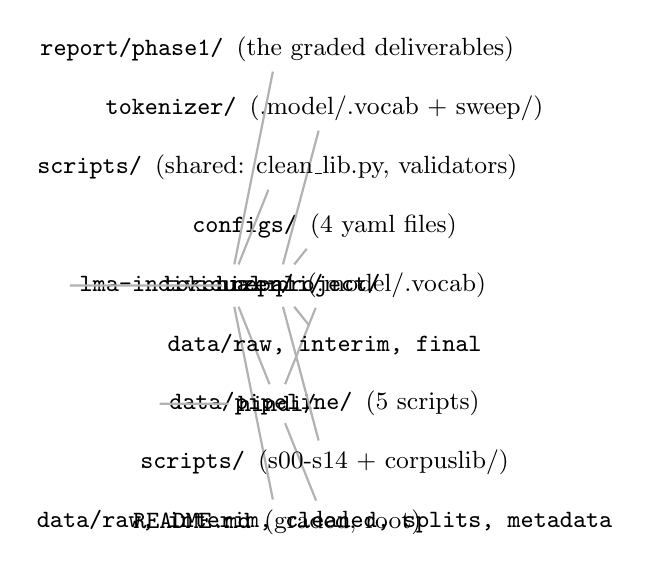
\begin{tikzpicture}[
  every node/.style={font=\ttfamily\small},
  level distance=6mm,
  edge from parent/.style={draw=gray!60, thick},
  grow=right,
]
\node {lma-individual-project/}
  child { node {README.md \textnormal{\rmfamily(graded, root)}} }
  child { node {hindi/}
    child { node {data/raw, interim, cleaned, splits, metadata} }
    child { node {data/pipeline/ \textnormal{\rmfamily(5 scripts)}} }
    child { node {tokenizer/ \textnormal{\rmfamily(.model/.vocab)}} }
  }
  child { node {nepali/}
    child { node {scripts/ \textnormal{\rmfamily(s00-s14 + corpuslib/)}} }
    child { node {data/raw, interim, final} }
    child { node {configs/ \textnormal{\rmfamily(4 yaml files)}} }
    child { node {tokenizer/ \textnormal{\rmfamily(.model/.vocab + sweep/)}} }
  }
  child { node {scripts/ \textnormal{\rmfamily(shared: clean\_lib.py, validators)}} }
  child { node {report/phase1/ \textnormal{\rmfamily(the graded deliverables)}} };
\end{tikzpicture}
\end{center}

\section{Where each stage's output actually lives}

\begin{center}
\begin{tabular}{lll}
\toprule
What & Hindi path & Nepali path \\
\midrule
Raw manual & \texttt{hindi/data/raw/manual/} & \texttt{nepali/data/raw/manual/} \\
Raw downloaded & \texttt{hindi/data/raw/downloaded/} & \texttt{nepali/data/raw/downloaded/} \\
Post-normalize & \texttt{hindi/data/interim/} & \texttt{nepali/data/interim/s03\_normalized/} \\
Per-stage snapshots & \textit{(single pass, no per-stage dirs)} &
\texttt{nepali/data/interim/s04\_langid/}, \texttt{s05\_heuristics/}, etc. \\
Final cleaned & \texttt{hindi/data/cleaned/} & \textit{(no single "cleaned" dir --
final output is} \texttt{data/final/} \textit{directly)} \\
Final splits & \texttt{hindi/data/splits/\{train,validation,test\}/} &
\texttt{nepali/data/final/\{train,val,test\}.jsonl} \\
Tokenizer & \texttt{hindi/tokenizer/*.model} & \texttt{nepali/tokenizer/*.model} +
\texttt{sweep/} \\
Stats/manifest & \texttt{hindi/data/metadata/clean\_stats.json} &
\texttt{nepali/data/final/corpus\_stats.json} \\
\bottomrule
\end{tabular}
\end{center}

\begin{warnbox}[Notice the naming difference]
Hindi's splits use the word \texttt{validation} (spelled out); Nepali's
use \texttt{val} (abbreviated). This is not a typo anywhere -- it's just
that the two pipelines were never unified, so their naming conventions
never got reconciled either. Both are correct within their own pipeline.
\end{warnbox}

% =======================================================================
\chapter{Deliverables Mapping}
% =======================================================================

This table is the direct answer to "which file satisfies which
requirement" -- exactly what a TA evaluation is likely to probe.

\begin{center}
\begin{longtable}{p{2.6cm}p{5.6cm}p{5.6cm}}
\toprule
\textbf{Requirement} & \textbf{Hindi} & \textbf{Nepali} \\
\midrule
\endhead
Dataset collection scripts &
\texttt{download\_hindi.py}, \texttt{ingest\_manual.py},
\texttt{ingest\_wikipedia\_dump.py} &
\texttt{s01\_collect.py} (driven by \texttt{collect.py}),
\texttt{auto\_grow\_and\_tokenize.py} \\
Preprocessing pipeline &
\texttt{clean\_hindi.py} + \texttt{scripts/clean\_lib.py} &
\texttt{s03}--\texttt{s10} (8 stage scripts) + \texttt{corpuslib} \\
Dataset statistics report &
\texttt{report/phase1/phase1\_report.md/.tex/.pdf}, \texttt{dataset\_
statistics.md}, \texttt{tokenizer\_analysis.md} (both languages, in one
combined report) & \textit{(same files, Nepali's own sections)} \\
Train/val/test splits &
\texttt{data/splits/\{train,validation,test\}/} + 3 manifest JSON files
(too large for git -- OneDrive) &
\texttt{data/final/\{train,val,test\}.jsonl} +
\texttt{split\_stats.json} (too large for git -- OneDrive) \\
Tokenizer training code &
\texttt{train\_tokenizer.py} &
\texttt{s12\_train\_tokenizer.py}, \texttt{s13\_tokenizer\_eval.py} \\
Vocabulary files &
\texttt{hindi\_unigram\_\{5000,8000,10000\}.vocab} (committed to git) &
\texttt{nepali\_bpe.vocab} + 4 swept sizes (committed to git) \\
Tokenizer model files &
\texttt{hindi\_unigram\_\{5000,8000,10000\}.model} (committed to git) &
\texttt{nepali\_bpe.model} + 4 swept sizes (committed to git) \\
\bottomrule
\end{longtable}
\end{center}

\begin{notebox}[Honest gap, stated plainly]
The actual split \textit{data files} (Hindi's manifests, Nepali's
\texttt{train.jsonl}/\texttt{val.jsonl}/\texttt{test.jsonl}) are
\textbf{not committed to git} for either language -- Hindi's train
manifest alone is 469MB, and Nepali's three split files total roughly
9.2GB. Both are correctly excluded from git per the course spec ("do not
commit large binary artifacts to git") and are meant to live on the
shared OneDrive link in the root README instead. One small exception:
Nepali's \texttt{split\_stats.json} is only 763 bytes and \textit{could}
be committed for free, but currently isn't, purely because it's caught
by the blanket \texttt{nepali/data/} gitignore rule.
\end{notebox}

% =======================================================================
\chapter{Running the Pipeline From Scratch}
% =======================================================================

\section{Hindi, step by step}

\begin{lstlisting}[language=bash]
python -m venv .venv
.venv/Scripts/activate
pip install -r requirements.txt

python hindi/data/pipeline/download_hindi.py
python hindi/data/pipeline/ingest_manual.py typed --input-dir <folder>
python hindi/data/pipeline/ingest_wikipedia_dump.py
python hindi/data/pipeline/clean_hindi.py
python hindi/data/pipeline/split_hindi.py
python hindi/tokenizer/train_tokenizer.py --vocab-size 8000
python hindi/tokenizer/analyze_tokenizer.py --vocab-size 8000
python scripts/validate_phase1.py
\end{lstlisting}

\textbf{How to verify each stage worked:} \texttt{clean\_hindi.py} prints
a summary (\texttt{docs\_cleaned/docs\_in}) and writes the full numbers
to \texttt{data/metadata/clean\_stats.json} -- read that file, don't just
trust the console. \texttt{validate\_phase1.py} at the end is the single
command that answers "is Phase 1 actually done" for Hindi -- it checks
all 4 required properties fresh from disk every time.

\section{Nepali, step by step}

\begin{lstlisting}[language=bash]
cd nepali/scripts
python s00_doctor.py                    # ALWAYS run this first
python auto_grow_and_tokenize.py        # runs S02-S14 in a loop until
                                         # both token targets are met
python ../../scripts/validate_phase1_nepali.py
python ../../scripts/check_nepali_hindi_overlap.py
\end{lstlisting}

Or, for finer control, run stages one at a time via
\texttt{run\_pipeline.py}:

\begin{lstlisting}[language=bash]
python run_pipeline.py pipeline              # S02 through S14, in order
python run_pipeline.py pipeline --from s08_dedup.py   # resume from one stage
\end{lstlisting}

\textbf{How to verify each stage worked:} every Nepali stage writes a
manifest JSON into its own \texttt{data/interim/<stage>/} folder with
\texttt{docs\_in}/\texttt{docs\_out}/\texttt{retention} -- read that, not
just the console output. \texttt{log.md} at the repo root accumulates one
human-readable entry per stage run across the whole project's history.

\section{Troubleshooting}

\begin{center}
\begin{tabular}{p{5.2cm}p{7.5cm}}
\toprule
\textbf{Symptom} & \textbf{What it means / what to do} \\
\midrule
\texttt{BLOCKED: ... has no stage manifest} &
The previous stage hasn't been run yet -- Nepali stages check this
explicitly before starting, rather than silently working on stale or
missing input. \\
\texttt{another process already holds <lock>} &
A previous run is still going, or died without cleaning up. If you're
sure nothing is actually running, the lock self-expires after 15
minutes, or delete the \texttt{.lock} file manually. \\
\texttt{BLOCKED: retention X\% outside expected [min, max]} &
S04 or S05 aborted \textit{on purpose} -- a retention rate this far from
expected is exactly the signature of the fastText/NumPy incident
(Section~5.3): inspect the sample files under
\texttt{data/interim/*\_samples/} before trusting the run, don't just
re-run and hope. \\
\texttt{no train text files found -- run split\_hindi.py first} &
Tokenizer training expects the splits to already exist; run the
preceding pipeline stage first. \\
Resume takes a very long time &
For Hindi, make sure \texttt{--resume} is actually being passed (a
fresh run without it rebuilds from scratch). For Nepali, S08's near-
duplicate pass is genuinely the slowest single stage in the whole
pipeline (measured at 30+ hours on one production run) -- this is not a
bug, MinHash/LSH over millions of documents is just expensive. \\
\bottomrule
\end{tabular}
\end{center}

% =======================================================================
\chapter{TA Evaluation Question Bank}
% =======================================================================

Each question below is grounded in this project's actual work. "Simple
answer" is what to say first, out loud; "Detailed answer" is the backup
if asked to go deeper.

\section{Theory}

\begin{qabox}{What is a corpus, and why does this project need two of
them?}
\textbf{Simple:} A corpus is just the large collection of text a
language model learns from. This project needs two, completely separate,
because it's training two independent models -- one per language -- and
the assignment forbids any sharing of data between them.\\
\textbf{Detailed:} Hindi's corpus (704,101 cleaned documents,
1.76B characters) and Nepali's (1,918,265 documents, 635M tokens) never
share a document, never share a tokenizer, and are built by two
completely different pipelines. This was explicitly verified: a
cross-language dedup check found 0 documents shared between them.\\
\textbf{Keywords:} corpus, monolingual, independence, cross-language check
\end{qabox}

\begin{qabox}{Why does Unicode normalization matter for this project?}
\textbf{Simple:} The same visual text can be stored as different byte
sequences in Unicode; normalizing picks one canonical form so duplicate
detection and cleaning actually work correctly.\\
\textbf{Detailed:} This project uses NFC, not NFKC, specifically because
NFKC can strip or alter ZWJ/ZWNJ characters that control real spelling
distinctions in Devanagari conjuncts -- using NFKC would silently corrupt
correctly-spelled Nepali/Hindi words.\\
\textbf{Keywords:} Unicode, NFC, NFKC, ZWJ, ZWNJ, Devanagari conjuncts
\end{qabox}

\begin{qabox}{Explain MinHash and LSH in your own words.}
\textbf{Simple:} MinHash turns a document into a short numeric
"fingerprint" such that similar documents get similar fingerprints. LSH
groups documents by fingerprint so only likely-similar documents ever get
compared directly, instead of comparing every document to every other
one.\\
\textbf{Detailed:} A document is broken into overlapping word-shingles;
100 different hash functions are applied and only the minimum result of
each is kept, forming a 100-number signature. Two documents' true
word-overlap similarity is approximated by what fraction of their
signature numbers match. LSH splits the signature into 20 bands of 5
numbers; documents are only compared if they share at least one full
band -- this makes near-duplicate detection scale to millions of
documents instead of requiring an all-pairs comparison.\\
\textbf{Keywords:} MinHash, LSH, shingle, Jaccard similarity, near-duplicate
\end{qabox}

\begin{qabox}{What's the difference between BPE and Unigram tokenization?}
\textbf{Simple:} BPE builds a vocabulary by repeatedly merging the most
frequent adjacent pair of tokens, and never undoes a merge. Unigram
starts from many candidate pieces and uses probability to prune down to
the target size, reconsidering the best segmentation for each piece of
text.\\
\textbf{Detailed:} BPE's greedy merging is fast but permanent -- an early
merge inside a bad boundary can't be revisited. Unigram treats
segmentation itself as probabilistic, which is argued (though not
empirically confirmed on this data) to suit Devanagari's morphologically
rich, conjunct-heavy structure better. This project uses both: Hindi uses
Unigram (a considered choice), Nepali uses BPE (this pipeline's
configured default), with an automatic fallback to also try Unigram if
BPE's fertility got too high (it never triggered for Nepali).\\
\textbf{Keywords:} BPE, Unigram, SentencePiece, subword tokenization,
fertility
\end{qabox}

\begin{qabox}{Why is data leakage between train and test a serious
problem?}
\textbf{Simple:} If test data (or something too similar to it) leaks
into training, evaluation results look better than the model's real
capability -- you're no longer measuring generalization to unseen data.\\
\textbf{Detailed:} This project guards against leakage at two levels:
document-level (never split by sentence, since that leaks context across
splits) and near-duplicate-level (Nepali's S09 decontamination stage
specifically removes train documents that are near-duplicates of
held-out val/test content, verified by a rescan finding zero remaining
matches).\\
\textbf{Keywords:} leakage, generalization, decontamination,
near-duplicate
\end{qabox}

\section{Pipeline}

\begin{qabox}{Why does Nepali's S07 (holdout) run before S05/S06 despite
the file numbers?}
\textbf{Simple:} If the same quality filters that pick training data also
get to curate the evaluation set, evaluation partly measures the
filters' own preferences instead of genuine model quality.\\
\textbf{Detailed:} S07 forks val/test out of the pool right after S04
(normalize + language-ID only). S05 (heuristics) and S06 (perplexity)
both read S07's leftover \texttt{train\_pool} output, never S04's output
directly -- so val/test are never touched by any quality-filtering
decision, keeping them a fair, unbiased sample of what was actually
collected.\\
\textbf{Keywords:} holdout, execution order, unbiased evaluation, train\_pool
\end{qabox}

\begin{qabox}{Walk through what happens to one document from collection
to being tokenizer training data, for Nepali.}
\textbf{Simple:} Collected $\to$ normalized $\to$ language-checked $\to$
(if selected for train) quality-filtered $\to$ perplexity-filtered $\to$
deduplicated $\to$ decontamination-checked $\to$ lane-balanced $\to$
written to \texttt{train.jsonl} $\to$ used to train the tokenizer.\\
\textbf{Detailed:} S01 collect $\to$ S03 normalize (NFC, doc\_id becomes a
content hash of normalized text) $\to$ S04 langid (fastText margin check)
$\to$ S07 assigns it to train/val/test by a seeded hash of its doc\_id
$\to$ if train: S05 heuristics $\to$ S06 perplexity $\to$ S08 exact+near
dedup $\to$ S09 decontamination check against held-out val/test $\to$ S10
lane balancing (only affects downloaded-lane documents) $\to$ S11 writes
it into \texttt{train.jsonl} $\to$ S12 trains the tokenizer using it.\\
\textbf{Keywords:} pipeline stages, doc\_id, content hash, stage order
\end{qabox}

\begin{qabox}{Why does Hindi's pipeline process manual documents before
downloaded ones?}
\textbf{Simple:} So that when two copies of the same text exist (one
manual, one downloaded), deduplication always keeps the manual copy.\\
\textbf{Detailed:} \texttt{clean\_hindi.py}'s \texttt{RAW\_DIRS} list is
explicitly \texttt{[raw/manual, raw/downloaded]}. Deduplication keeps
the first-seen copy of a duplicate hash and drops later ones -- so this
ordering is what guarantees a manual/downloaded collision always resolves
in favor of manual, protecting the scarce resource that the 20\% floor
is measuring. Nepali achieves the same guarantee differently: its dedup
stage explicitly checks lane and prioritizes manual regardless of
processing order.\\
\textbf{Keywords:} dedup priority, manual lane, RAW\_DIRS ordering
\end{qabox}

\begin{qabox}{What does \texttt{s00\_doctor.py} actually protect against?}
\textbf{Simple:} A silent environment bug that once deleted 94\% of a
corpus while logging "SUCCESS."\\
\textbf{Detailed:} \texttt{fasttext} crashed on a NumPy version
incompatibility; the crash was caught by a blanket \texttt{except
Exception} and treated as "document rejected," so nearly the whole corpus
was silently thrown away over four hours, with the run reporting success
throughout. \texttt{s00\_doctor.py} now tests every dependency actually
works \textit{before} any expensive stage runs, and the retention-band
abort in S04/S05 is the second layer of defense against the same failure
mode recurring in a different form.\\
\textbf{Keywords:} silent failure, fastText, NumPy, retention band, fail loudly
\end{qabox}

\section{Code and files}

\begin{qabox}{What is \texttt{corpuslib}, and why does it exist as a
separate package?}
\textbf{Simple:} It's the shared code every Nepali pipeline stage
imports -- config loading, JSONL I/O, dedup math, language ID, etc. --
kept in one place so 15 stage scripts don't each reimplement the same
logic.\\
\textbf{Detailed:} Modules include \texttt{config.py} (loads YAML
configs into one object), \texttt{stageio.py} (reads/writes a stage's
JSONL + manifest), \texttt{dedup.py} (MinHash/LSH, used by both S08 and
S09), \texttt{langid.py}, \texttt{heuristics.py}, \texttt{ngramlm.py}. It
was originally designed to be shared between both languages (with Hindi
as the intended "source of truth" copy, per the \texttt{sync}
subcommand in \texttt{run\_pipeline.py}), but only Nepali actually uses
it in this repo.\\
\textbf{Keywords:} corpuslib, shared library, stageio, config loading
\end{qabox}

\begin{qabox}{What does \texttt{scripts/validate\_phase1.py} actually
check?}
\textbf{Simple:} Four things for Hindi: raw manual+downloaded sources
exist, manual share is at least 20\%, splits exist with no overlap, and
a tokenizer has been trained.\\
\textbf{Detailed:} Each check reads real files (never a hardcoded count):
\texttt{raw/\{manual,downloaded\}/metadata.jsonl} for source presence,
\texttt{cleaned/metadata.jsonl}'s \texttt{source\_type} field for the
manual percentage, the three split manifests for a document-id
intersection check, and a glob for any \texttt{.model} file. It
originally also checked a Hindi$\leftrightarrow$Bhojpuri cross-language
overlap; that check was removed once Bhojpuri's files were deleted from
the repo (Nepali has its own separate cross-language script against
Hindi instead).\\
\textbf{Keywords:} validator, PASS/FAIL, manual floor, no-leakage check
\end{qabox}

\begin{qabox}{Where is the manual-vs-downloaded distinction actually
recorded in the data?}
\textbf{Simple:} A \texttt{source\_type} field ("manual" or "downloaded")
on every single document's metadata, from the moment it's collected.\\
\textbf{Detailed:} This field is written at collection time (e.g.\
\texttt{download\_hindi.py} always writes \texttt{source\_type=
"downloaded"}; \texttt{ingest\_manual.py} always writes
\texttt{"manual"}) and survives unchanged all the way through cleaning
into the final corpus, which is what lets the manual percentage be
recomputed directly from real files at any time rather than trusted as a
remembered number.\\
\textbf{Keywords:} source\_type, metadata, provenance, manual percentage
\end{qabox}

\section{Data and design decisions}

\begin{qabox}{Why absolute token targets instead of a manual/downloaded
ratio for Nepali?}
\textbf{Simple:} A ratio target conflates "how much text exists" with
"what fraction is manual" -- an earlier version of this exact idea
threw away a huge amount of good downloaded text just to hit a
percentage, when the manual lane was genuinely small.\\
\textbf{Detailed:} Chasing a ratio (e.g.\ "manual must be 24\% of
total") when manual was only 5.82\% forced cutting downloaded from 209.8M
words to 41.1M -- destroying volume to satisfy a percentage. This
project's actual approach: two independent absolute targets (manual
$\geq$ 100M tokens, downloaded $\geq$ 400M tokens). Manual is kept at
100\% always; downloaded is trimmed to its own target; if manual still
falls short, that's a signal to collect more manual data, never a reason
to cut downloaded further.\\
\textbf{Keywords:} absolute target, ratio, lane balancing, S10
\end{qabox}

\begin{qabox}{Why is Nepali's manual share reported as token-weighted
while Hindi's is char-weighted?}
\textbf{Simple:} Because Nepali's pipeline never added per-lane character
tracking -- token-weighted is the real, honest number that's actually
available for it.\\
\textbf{Detailed:} This is disclosed explicitly in the report rather
than hidden or forced into a false apples-to-apples comparison. It's one
of several genuine methodology differences between the two pipelines
(see also: different dedup methods, different tokenizer algorithms).\\
\textbf{Keywords:} token-weighted, char-weighted, methodology difference
\end{qabox}

\begin{qabox}{Why does this project not use a pretrained tokenizer or
model?}
\textbf{Simple:} The assignment explicitly forbids it -- the entire point
of the exercise is to build everything from scratch to demonstrate real
understanding.\\
\textbf{Detailed:} No pretrained language models, no pretrained
tokenizers, no HuggingFace model classes are allowed anywhere in this
project, for either phase. This is why even the tokenizer training
(SentencePiece) starts from raw cleaned text with no prior vocabulary,
rather than extending or fine-tuning an existing one.\\
\textbf{Keywords:} from-scratch, no pretrained models, assignment constraint
\end{qabox}

\section{Hindi-specific}

\begin{qabox}{Why does Hindi's cleaning pipeline have a Bhojpuri-marker
check at all?}
\textbf{Simple:} Because \texttt{langdetect} (the library Hindi's
pipeline uses) has no label for Bhojpuri, so it would happily call real
Bhojpuri text "Hindi" -- the marker check catches what the library
structurally cannot.\\
\textbf{Detailed:} \texttt{clean\_lib.py}'s \texttt{marker\_counts()}
counts occurrences of common Bhojpuri words (\dn{बा}, \dn{बाटे},
\dn{गइल}, etc.) versus common Hindi words (\dn{है}, \dn{हैं}, \dn{गया},
etc.); if Bhojpuri markers clearly outnumber Hindi markers, the document
is rejected as \texttt{likely\_bhojpuri} \textit{before}
\texttt{langdetect} even runs. This filter predates and is independent
of Bhojpuri's later removal as Model L -- it's part of Hindi's own
cleaning history and still runs today, even though the risk it originally
guarded against (accidentally training Hindi on the language that used to
be this project's own Model L) no longer applies day to day.\\
\textbf{Keywords:} likely\_bhojpuri, marker\_counts, langdetect limitation
\end{qabox}

\begin{qabox}{What was the Hindi$\leftrightarrow$Bhojpuri cross-language
incident, exactly?}
\textbf{Simple:} 2 documents were found to be genuinely Bhojpuri text
that an upstream dataset (Sangraha) had mislabeled as Hindi; both were
removed from Hindi's cleaned corpus with a small, targeted, one-time
script.\\
\textbf{Detailed:} \texttt{validate\_phase1.py}'s cross-language check
(while Bhojpuri was still Model L) found 2 documents sharing a content
hash between the Hindi and Bhojpuri cleaned corpora. Both contained
Bhojpuri-specific verb forms not in Hindi's marker list, and had been
sourced as \texttt{hin} by \texttt{ai4bharat/sangraha} while correctly
labeled \texttt{bho\_Deva} by \texttt{HuggingFaceFW/fineweb-2} for the
same underlying text -- an upstream labeling error, not a bug in this
project's pipeline. \texttt{scripts/remove\_cross\_language\_duplicates.py}
removed them, which is why Hindi's final count is 704,101, not
\texttt{clean\_stats.json}'s own recorded 704,103.\\
\textbf{Keywords:} cross-language contamination, upstream labeling error,
704101 vs 704103
\end{qabox}

\section{Nepali-specific}

\begin{qabox}{Why does Nepali use BPE if the theoretical argument (in this
project's own Hindi section) favors Unigram for Devanagari?}
\textbf{Simple:} Because BPE was this pipeline's configured default,
chosen independently before that Hindi-specific argument was written up
-- not a per-language linguistic decision. There's a real safety net
though: a comparison to Unigram would have kicked in automatically if
BPE's fertility got too high, and it simply never needed to.\\
\textbf{Detailed:} \texttt{nepali/configs/tokenizer.yaml} sets
\texttt{model\_type: bpe} with
\texttt{compare\_unigram.trigger\_fertility\_above: 2.10}. Nepali's
measured BPE fertility across the whole sweep (1.48--1.70) never came
close to that threshold, so the automatic Unigram comparison never
triggered. This is a real, working comparison mechanism that happened not
to change the outcome -- not an untested assumption.\\
\textbf{Keywords:} BPE vs Unigram, compare\_unigram, fertility threshold
\end{qabox}

\begin{qabox}{Why did Nepali's pipeline run on a separate machine?}
\textbf{Simple:} The MinHash/LSH near-duplicate dedup stage (S08) alone
took over 30 hours on this project's primary machine, which wasn't
practical within the deadline window.\\
\textbf{Detailed:} Only the pipeline's output artifacts were transferred
back into this repository, not live per-stage console logs -- so
\texttt{log.md}'s later-stage entries for Nepali (S08 production run
onward) are reconstructed after the fact from those output files, which
is disclosed explicitly in the log itself rather than presented as if it
were live-logged.\\
\textbf{Keywords:} provenance, separate machine, reconstructed log entries
\end{qabox}

\begin{qabox}{Why was Bhojpuri replaced by Nepali as Model L?}
\textbf{Simple:} Bhojpuri was fully built and passed every check, but its
real available public data is genuinely small (its final corpus reached
only 16.8\% of the 500M-token target, a documented and spec-permitted
shortfall). Nepali had enough available public data to clear the same
target comfortably, and once its own pipeline was finished, it replaced
Bhojpuri.\\
\textbf{Detailed:} Bhojpuri's shortfall was not a collection-effort
problem -- every known manual source was recrawled and confirmed
exhausted, and every findable Bhojpuri-labeled Hugging Face dataset was
evaluated. Nepali's larger public-data availability (via AI4Bharat's
Sangraha and IndicCorpV2) let it reach 127.0\% of target instead. This
was a deliberate, disclosed switch, not a quiet substitution --
Bhojpuri's own numbers remain in the report as history, and its code has
since been removed from the repository, but nothing about that history is
hidden.\\
\textbf{Keywords:} Model L switch, Bhojpuri shortfall, spec-permitted
\end{qabox}

\section{Limitations}

\begin{qabox}{What is the single biggest acknowledged weakness in this
project's cleaning?}
\textbf{Simple:} Hindi's language-ID/contamination check is a hand-written
lexical marker list, not a trained classifier -- it will not catch every
case, and the cross-language incident (2 leaked documents) is proof it
already missed some.\\
\textbf{Detailed:} The report states this honestly rather than
overselling the filter's reliability: a coarse lexical heuristic can only
ever be a partial defense. Given more time, a real trained classifier
would be the first thing to build instead.\\
\textbf{Keywords:} lexical heuristic, known limitation, trained classifier
\end{qabox}

\begin{qabox}{What's the biggest structural difference between the two
pipelines that was never reconciled?}
\textbf{Simple:} Near-duplicate detection -- Hindi only does exact-hash
dedup; Nepali runs full MinHash/LSH near-duplicate detection. This is a
real asymmetry, not a shared gap.\\
\textbf{Detailed:} Hindi's pipeline was built first and never had
MinHash/LSH added to it, even after Nepali's pipeline demonstrated it
works. Given more time, this would be a natural next improvement for
Hindi's pipeline specifically.\\
\textbf{Keywords:} exact-hash, MinHash, pipeline asymmetry
\end{qabox}

% =======================================================================
\chapter{Cheat Sheet}
\label{chap:limitations}
% =======================================================================

\section{Numbers to have memorized}

\begin{center}
\begin{tabular}{lrr}
\toprule
& \textbf{Hindi (Model H)} & \textbf{Nepali (Model L)} \\
\midrule
Final tokens & 505,852,028 (101.2\%) & 635,204,333 (127.0\%) \\
Final documents & 704,101 & 1,918,265 \\
Manual share & 28.65\% (char) & 26.41\% (token) \\
Train/val/test & 675,937/14,082/14,082 & 1,520,000/199,428/198,837 \\
Tokenizer & Unigram, vocab 8,000 & BPE, vocab 10,000 \\
Dedup method & exact-hash only & exact-hash + MinHash/LSH \\
Cross-language overlap & \multicolumn{2}{c}{0 shared documents (verified)} \\
\bottomrule
\end{tabular}
\end{center}

\section{File names to have memorized}

\begin{center}
\begin{tabular}{ll}
\toprule
Hindi & Nepali \\
\midrule
\texttt{download\_hindi.py} & \texttt{s01\_collect.py} / \texttt{collect.py} \\
\texttt{clean\_hindi.py} + \texttt{clean\_lib.py} & \texttt{s03}--\texttt{s10} + \texttt{corpuslib/} \\
\texttt{split\_hindi.py} & \texttt{s07\_holdout.py} + \texttt{s11\_finalize\_splits.py} \\
\texttt{train\_tokenizer.py} & \texttt{s12\_train\_tokenizer.py} \\
\texttt{analyze\_tokenizer.py} & \texttt{s13\_tokenizer\_eval.py} \\
-- & \texttt{auto\_grow\_and\_tokenize.py} (outer loop) \\
\texttt{scripts/validate\_phase1.py} & \texttt{scripts/validate\_phase1\_nepali.py} \\
\bottomrule
\end{tabular}
\end{center}

\section{Pipeline stage order to recite}

Nepali: \textbf{S00 doctor $\to$ S01 collect $\to$ S02 calibrate $\to$ S03
normalize $\to$ S04 langid $\to$ S07 holdout $\to$ S05 heuristics $\to$
S06 perplexity $\to$ S08 dedup $\to$ S09 decontaminate $\to$ S10 balance
lanes $\to$ S11 finalize splits $\to$ S12 train tokenizer $\to$ S13
tokenizer eval $\to$ S14 corpus stats.} Remember: S07 runs out of order,
right after S04, before S05/S06 -- this is the single most-likely-to-
be-asked-about sequencing detail in this whole project.

Hindi: \textbf{download $\to$ ingest (manual + Wikipedia dump) $\to$
clean $\to$ split $\to$ train tokenizer $\to$ analyze tokenizer.} No stage
numbering, no orchestrator script -- run by hand, in this order.

\section{Design decisions to be ready to defend}

\begin{itemize}[leftmargin=*]
\item Manual copy always wins a manual/downloaded duplicate tie --
protects the scarce resource the 20\% floor measures.
\item Absolute token targets (Nepali), not a manual/downloaded
\textit{ratio} -- avoids conflating volume with composition.
\item Val/test held out \textit{before} quality filtering (Nepali S07) --
keeps evaluation unbiased by the filters' own preferences.
\item NFC, never NFKC -- preserves real Devanagari spelling
(ZWJ/ZWNJ matter).
\item Document-level splits, never sentence-level -- prevents leakage.
\item Fail loudly, not silently -- S00/S04/S05's abort-on-bad-retention
behavior exists because of a real incident that deleted 94\% of a corpus
under a "SUCCESS" log.
\end{itemize}

\section{One-sentence summary, if asked "what did you actually build in
Phase 1?"}

\begin{tcolorbox}[colback=titlenavy!5,colframe=titlenavy,fonttitle=\bfseries,
coltitle=white,colbacktitle=titlenavy,title={Recite this}]
"I built two independent data pipelines -- Hindi's is a single-pass
cleaner, Nepali's is a 15-stage pipeline with its own dedup and quality
filters -- that together turned 3.4 million raw documents into two
clean, split, tokenized corpora totaling over 1.1 billion tokens, both
clearing the 20\% manual-collection floor, with zero content overlap
between the two languages, verified end to end."
\end{tcolorbox}

% =======================================================================
\chapter{Honest Limitations Summary}
\label{sec:limitations-summary}
% =======================================================================

This chapter exists so nothing is quietly overstated. All of these are
also disclosed in the actual graded report.

\begin{itemize}[leftmargin=*]
\item \textbf{Hindi has no near-duplicate detection}, only exact-hash --
Nepali's MinHash/LSH capability was never retrofitted onto Hindi's
pipeline.
\item \textbf{Hindi's Unigram-vs-BPE argument is structural, not
empirically tested} on Hindi's own data specifically.
\item \textbf{The Bhojpuri-contamination marker list is a coarse
heuristic}, not a trained classifier, and is known to have missed real
cases (the 2-document cross-language incident).
\item \textbf{Nepali's manual share is token-weighted}, not
char-weighted like Hindi's -- a genuine methodology difference, not an
oversight glossed over.
\item \textbf{Nepali's SentencePiece sampled-character count was not
logged} by its pipeline the way Hindi's was -- a real reporting gap.
\item \textbf{The cross-language overlap check only covers Nepali vs.\
Hindi}, not Nepali vs.\ Bhojpuri, since Bhojpuri is no longer part of the
submission.
\item \textbf{Whether the large data files are actually uploaded to
OneDrive} (as opposed to just existing locally) was not independently
verifiable at the time of writing this project's documentation.
\item \textbf{No neural network architecture exists yet.} Phase 1 is data
and tokenizer only -- this is by design, not an oversight, but worth
stating plainly if asked.
\end{itemize}

\end{document}
